\documentclass{DeustoFDP}
\usepackage{hologo} % Paquete no necesario. Borrar en la memoria final al sustituir el texto
\hypersetup{
pdfauthor={Aitor Brazaola Vicario},
pdftitle={Final Degree Project - Aitor Brazaola. University of Deusto},
}

\bibliography{bib}

\begin{document}

\frontmatter
\pagestyle{plain}

% Las siguientes lineas (21--26) se pueden eliminar del documento final.
% Notese que en ese caso es necesario descomentar la linea 28 para que las
% paginas esten correctamente numeradas.
\begin{titlepage}
    \newgeometry{left=0cm,right=0cm,bottom=0cm,top=0cm}
    
\includegraphics{fig/portada}
    \restoregeometry
\end{titlepage}
\cleardoublepage

\setcounter{page}{3}

\chapter*{Abstract}
The lifestyle of today's society moves away the contact between neighbors
which has always existed in all communities in which it promotes the
exchange of goods, favors and often vital information for all
the inhabitants of the community. In addition, the growth of cities makes
that meeting the needs and concerns of the inhabitants ever be a
more difficult for municipalities task.

Auzonet as digital platform focused on the residents, provides
the perfect setting to neighbors having a web platform
to exchange all this information and the organizations as data source.

\vspace{2em}

{\Large\bfseries\sectionfont Keywords}
\vspace{3\medskipamount}

OpenData, Web, App, Social network.

\cleardoublepage\tableofcontents
\cleardoublepage\listoffigures
\cleardoublepage\listoftables
\cleardoublepage\listoflistings

\mainmatter
\pagestyle{phdthesis}

\chapter{Introduction}\label{cha:introduction}
The aim of this project is to create an online social platform that benefits different parties, on the one hand, the residents themselves having a common point of meeting in the community  through internet where they can post notices or information corresponding permanently to the community in a virtual cork, simile of physics that normally exists in doorways, and to publish requests or offers of items or services allowing interaction of stakeholders across the platform.

On the other hand, the information generated by the use of the platform can be a source of high-quality data for services of the municipalities, so that, analyzing these decisions can be made based on the real needs predominate more in each neighborhood.

This project must be developed on the basis of European project ~\cite{WeLive} which ~\cite{DeustoTech} ~\cite{Morelab} belongs to, using the libraries and programming interfaces that makes available. WeLive is a web platform for the promotion of OpenData created by several European entities that provides a range of services for developers and public entities for the purpose of data dissemination and exploitation of them in third-party applications at no cost.

The main challenges will tackle this project are:

\begin{itemize}
    \item Creating a social web portal with the required functions.
    \item The exploitation of public datasets that add value to the application.
    \item The creation of new datasets depending on the spindle.
    \item Creating a mobile application able to interact with fellow on the web through an interface.
\end{itemize}

In addition, during development they may be needed to develop new software components that allow customized integration with WeLive and can be reused in future projects by making them publicly available in the application repository of WeLive.

This project will need technical ability and interpersonal skills to achieve good collaboration between teams WeLive and create Auzonet to achieve the best possible solution.

To carry out major development of the application, it will use a web framework that allows implement most of the functions of the web application with maximum code reuse and greater efficiency, as when developed mobile application, is going to be necessary a framework that allows the development at the same time for all operating systems currently on the market.

The previously mentioned tools add the challenge of conducting an investigation about the  mobile web development frameworks and learning the model of communication that requires WeLive to interact with public data .

All phases of development will demonstrate exhaustively the knowledge acquired during the university degree and also require new learning, both technical and theoretical knowledge.

This document describes the project and make an approach to the most similar solutions exist today and will discuss the importance of Open Data and what it brings to society, the WeLive project will be described and all possibilities that offers.

After, planning and development process will be described.

In the development chapter the internal development process will de explained, reasoning tools finally have been used and the reasons for their choice and the structure of the project and possible functional divisions of software components, design and requirements.


Finally, the conclusions found throughout the entire process of creation and information will be taken about the use in tests scheduled for future projects will be presented.

\chapter{Background and rationale}
\section{Background}
Creating a social network of neighbors in which all members of each portal or community can interact with each other by sharing resources and information is not a new initiative, in other countries like Germany or United States similar projects \cite{larazon} have been developed, internet has extended the creation of communities of all kinds of areas, however, the already existing proposals rarely get benefit of the public entities data, and in many cases, they are the most reliable source of information for building applications and services for citizens.

Although it is true that currently, many public entities make available this data in digital format only by the look of transparency and are unaware of the true value of themselves, is one of the motivation of this project, in fact, have been moments during the development in which the data found poorly formatted and have had to request modifications to the agencies involved.

The fact that most of datasets that are published by public organizations are not used in systems created by third parties, causes certain unconcern in the status and integrity of them.

\section{Rationale}
This project aims to unify the capabilities of communication between people that internet provides with the benefits of the Open Data to citizens, something that rarely have been done in similar intiatives.

\chapter{Goals and scope}
\section{Project definition}
Auzonet must meet the expectations of at least two types of users:
\begin{description}
	\item[Citizen:] It is the primary user of the system and the beneficiary of the features offered by the platform and the source of the information that the system creates for later exploitation.
	\item[Public institution:] It who analyze the data generated by the platform for statistics and promoting services that improve the quality of life in cities and people.
\end{description}

To achieve this it will develop:
\begin{itemize}
	\item A web application where users can register their neighborhood based on existing data published by the council of Bilbao, the rest of neighbors interested can join to it and get benefit from its functions.
	
	\item A mobile application that lets you interact with the main functions of the web from a smartphone.
\end{itemize}

\subsection{Functionality}
Users can search their portal trough an interactive form based on the existing neighbors and streets of the city of Bilbao, for better confirmation of the place, a small map showing the exact situation of the door will be displayed, if the information is correct, a few setting should be configure like the privacy level of the community having the option to protect it with a password or add a few lines of welcome message to new members via mail.

Each user can belong to more than one community of neighbors, considering that may want to be aware of the community of their usual residence and for example the holidays.

Each neighborhood community represented in the application has its own home page where you can see the cork with warnings or information notes published and a lower table divided into two sections called Requests and Offers where will be displayed the posts created by members of that community.

From the home page of each community, the user can create a request for a product or service or to publish an offer in which can specify whether you want to get paid or offer the service for free.

To ensure some confidence when working with another user, a karma level system represented by a numeric value that is higher or lower by other users past reviews determine the trust level of each user.

\subsection{Limitations}
Auzonet never going to manage payments among individuals, beyond the simple fact of a history of interactions between requests and offers between neighbors. Interested parties should agree on a transaction which methods used to pay if they require and have the complete responsibility for ensuring the successful transaction in a legal economic frame.

Will be the users themselves who in case to use the platform will have to register their portal in the section for creating communities to make use of the software functions.

There are no plans to develop applications with the native development kit of each mobile operating system for avoiding multiple processes of simultaneous development during the creation of the mobile application, web technologies to deploy the application available on the market will be used.

\section{Description of the embodiment}
\subsection{Development methodology}
The realization of Auzonet is separated in two main functional units, first will focus on finalizing the web application and then mobile app.

As can be seen in the figure \ref{fig:edt} the development phases are going to be the following:
\begin{description}
	\item[Requirements:] Analysis of the main functional requirements.
	\item[Design:] Design data and logical structures needed for running the application and approach to the aesthetic design of the solution.
	\item[Web application development:] Implementation process of the main application, with Welive project integration and "responsive" design for fitting on different screen sizes.
	\item[Mobile application development:] Implementation process of mobile application that get benefits of the "responsive" design of the web application.
	\item[Tests:] Different executions by end users and bug detection on the feature usage processes for debugging, It will try to involve collaborators and friends of the programmer for making real usage of the platform.
\end{description}

Being a project that involves only one developer will not be used agile methodologies that facilitate cooperation and teamwork, instead, a system of lists of tickets with different classifications will be used in a task manager software.

Tasks are classified as follows:
\begin{table}[H]
	\centering
	\caption{Ticket categories.}\label{tab:ticketcategories}
	\begin{tabular}{cccc}
		\toprule
		\textbf{Category} & \emph{Description}\\
		\midrule
		Functional  & Features that represent the core of the application.\\
		Not functional   & Features that enrich the user experience.\\
		Bug & Faults to debug.\\
		Improvement & Suggestions or new functionalities that add value to the platform.\\
		\bottomrule
	\end{tabular}
\end{table}

Sometimes, certain tasks can come from external sources such as suggestions for improvement or major deficiencies found in a test, in that case, they are added to the list with the corresponding label and prioritized according to their importance.
\subsection{Intermediate products}
\begin{itemize}
	\item Web application.
	\item Public data integrated via WeLive platform.
	\item Mobile application.
\end{itemize}
\newpage
\begin{figure}[H]
	\centering
	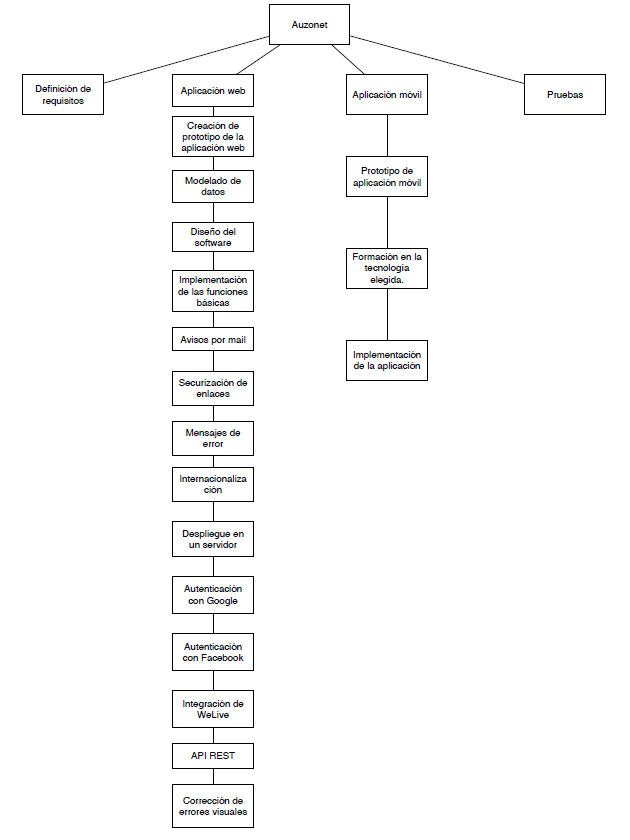
\includegraphics{fig/EDT}
	\caption{EDT}\label{fig:edt}
\end{figure}
\subsection{Main tasks}
\begin{figure}[H]
	\centering
	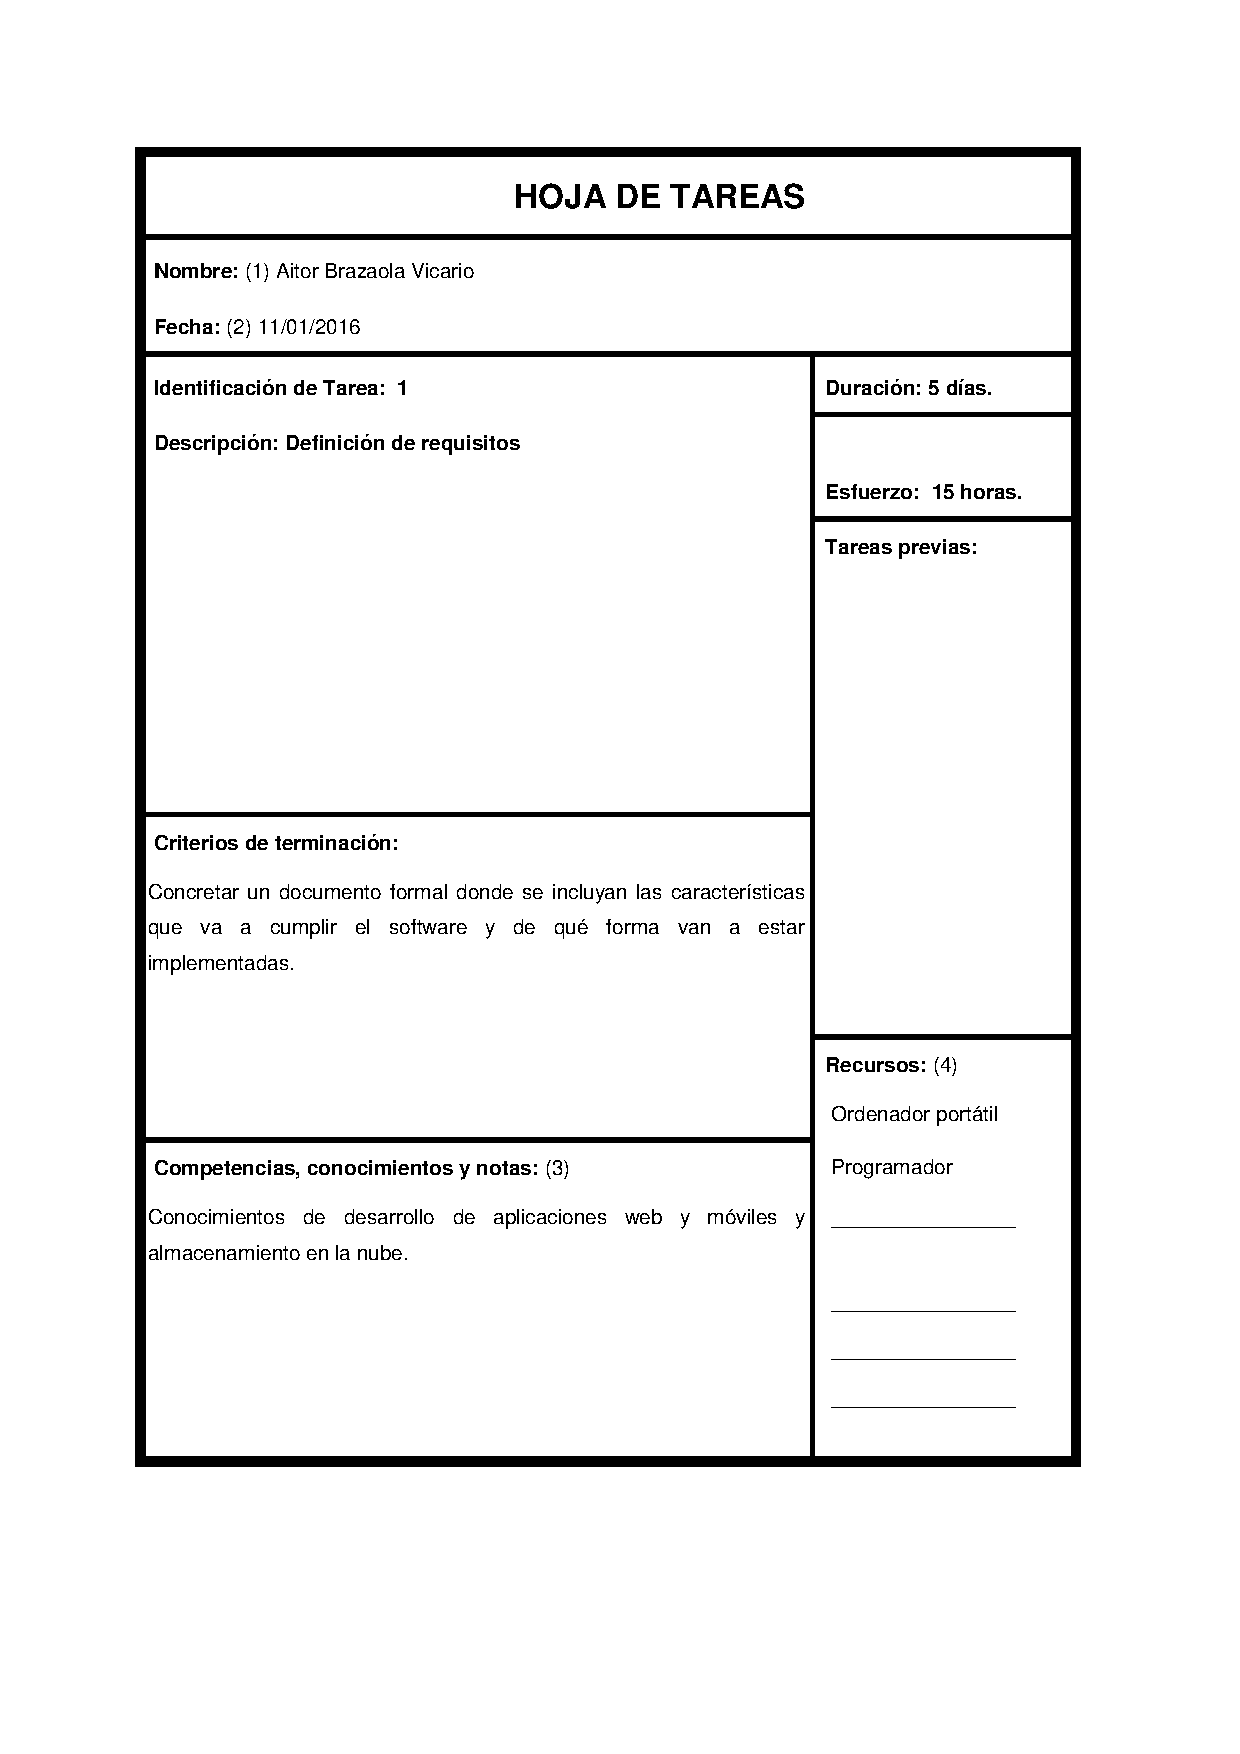
\includegraphics[width=0.9\textwidth]{fig/Tareas/1}
	\caption{Task 1}
	\label{fig:t1}
\end{figure}

\begin{figure}[H]
	\centering
	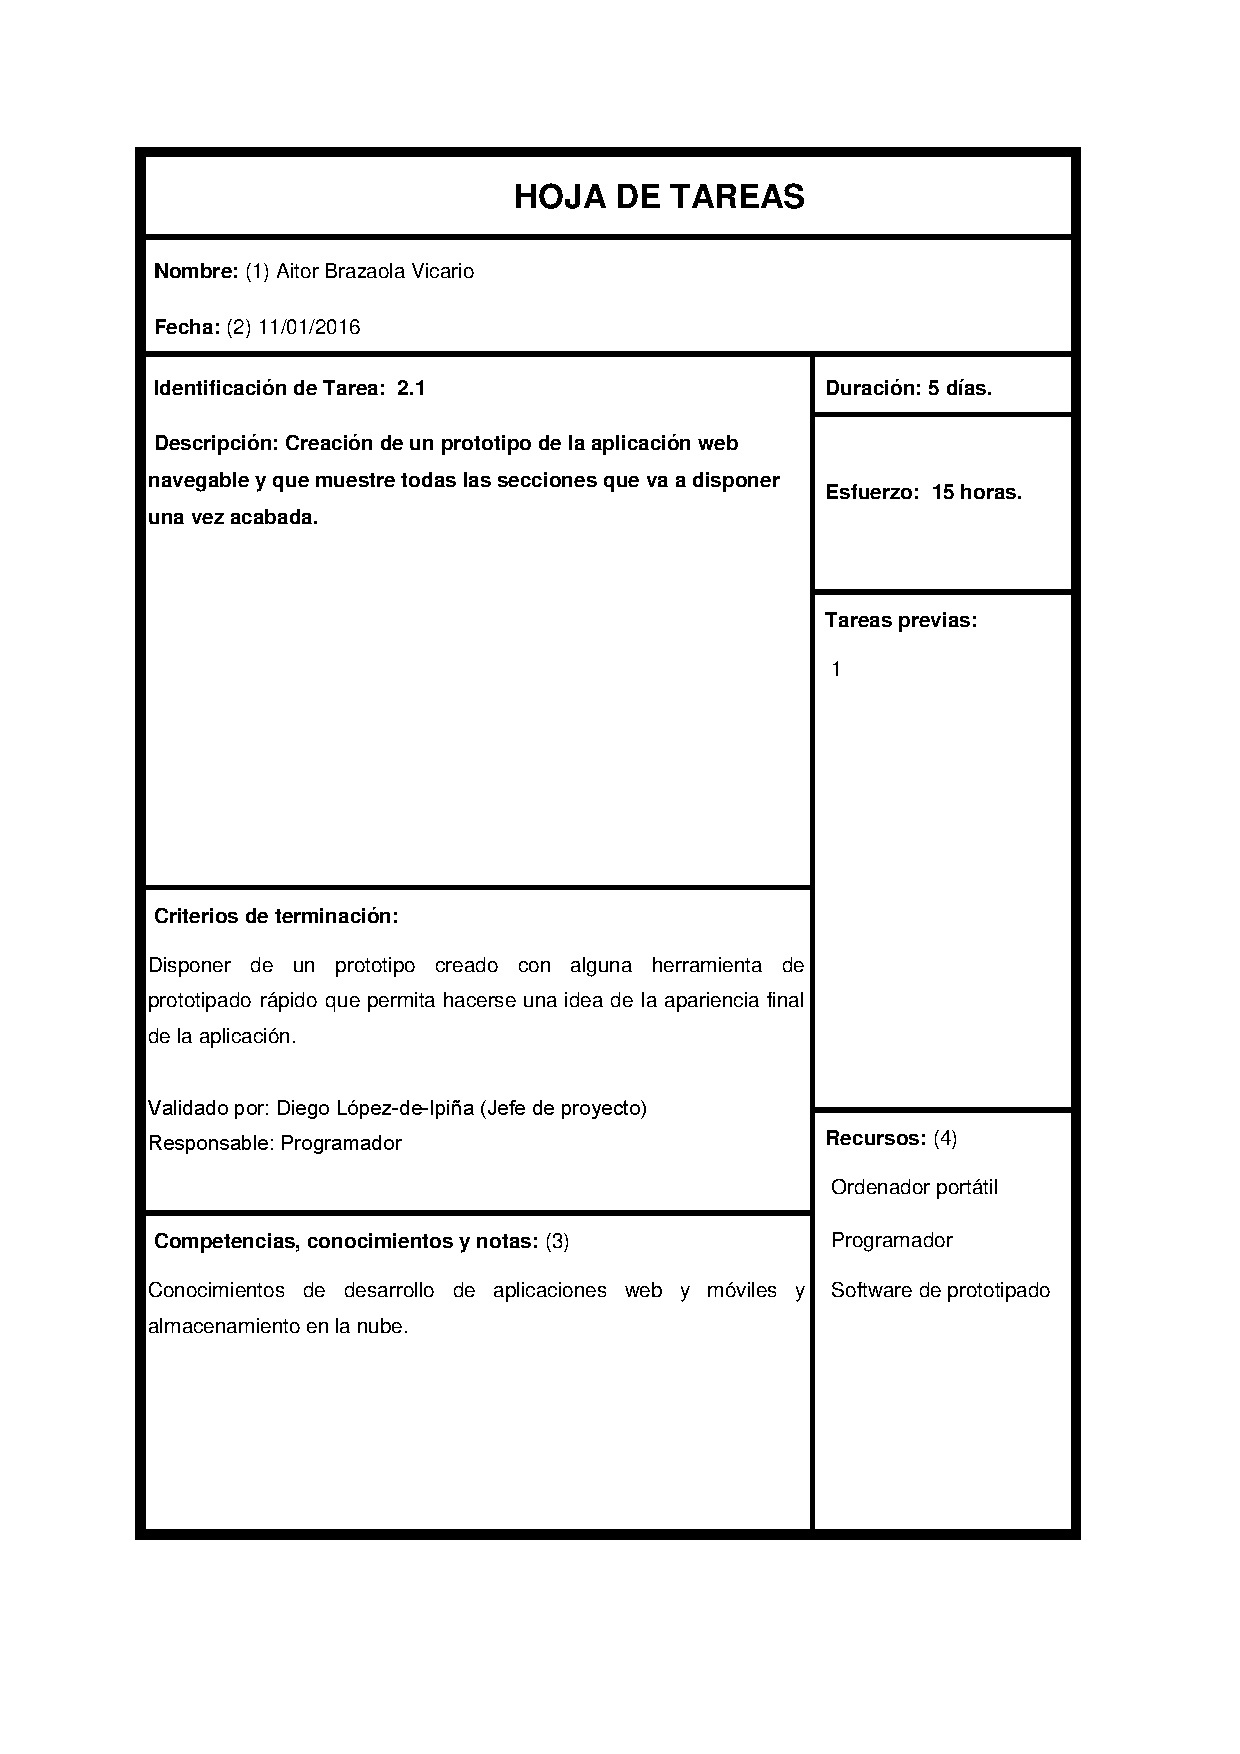
\includegraphics[width=0.9\textwidth]{fig/Tareas/21}
	\caption{Task 2.1.}
	\label{fig:t21}
\end{figure}

\begin{figure}[H]
	\centering
	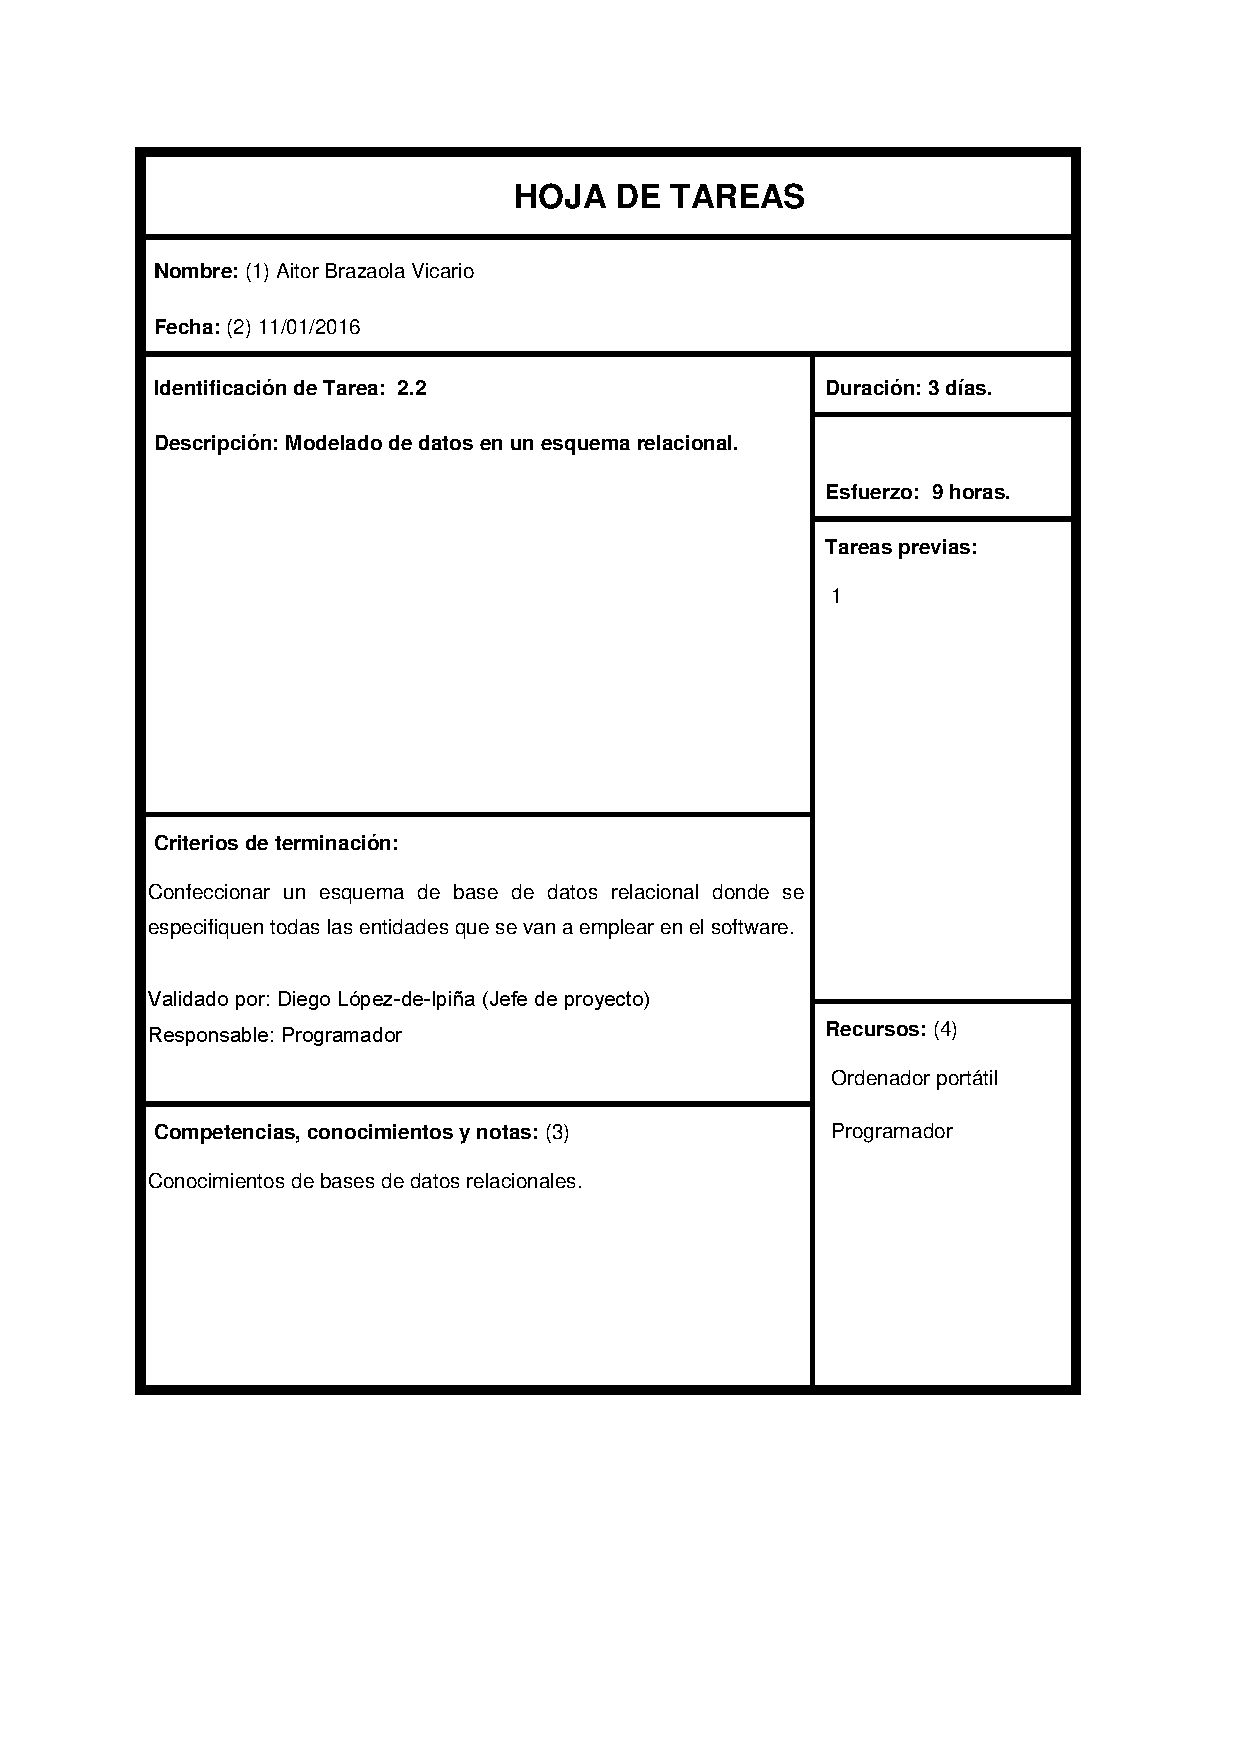
\includegraphics[width=0.9\textwidth]{fig/Tareas/22}
	\caption{Task 2.2.}
	\label{fig:t22}
\end{figure}

\begin{figure}[H]
	\centering
	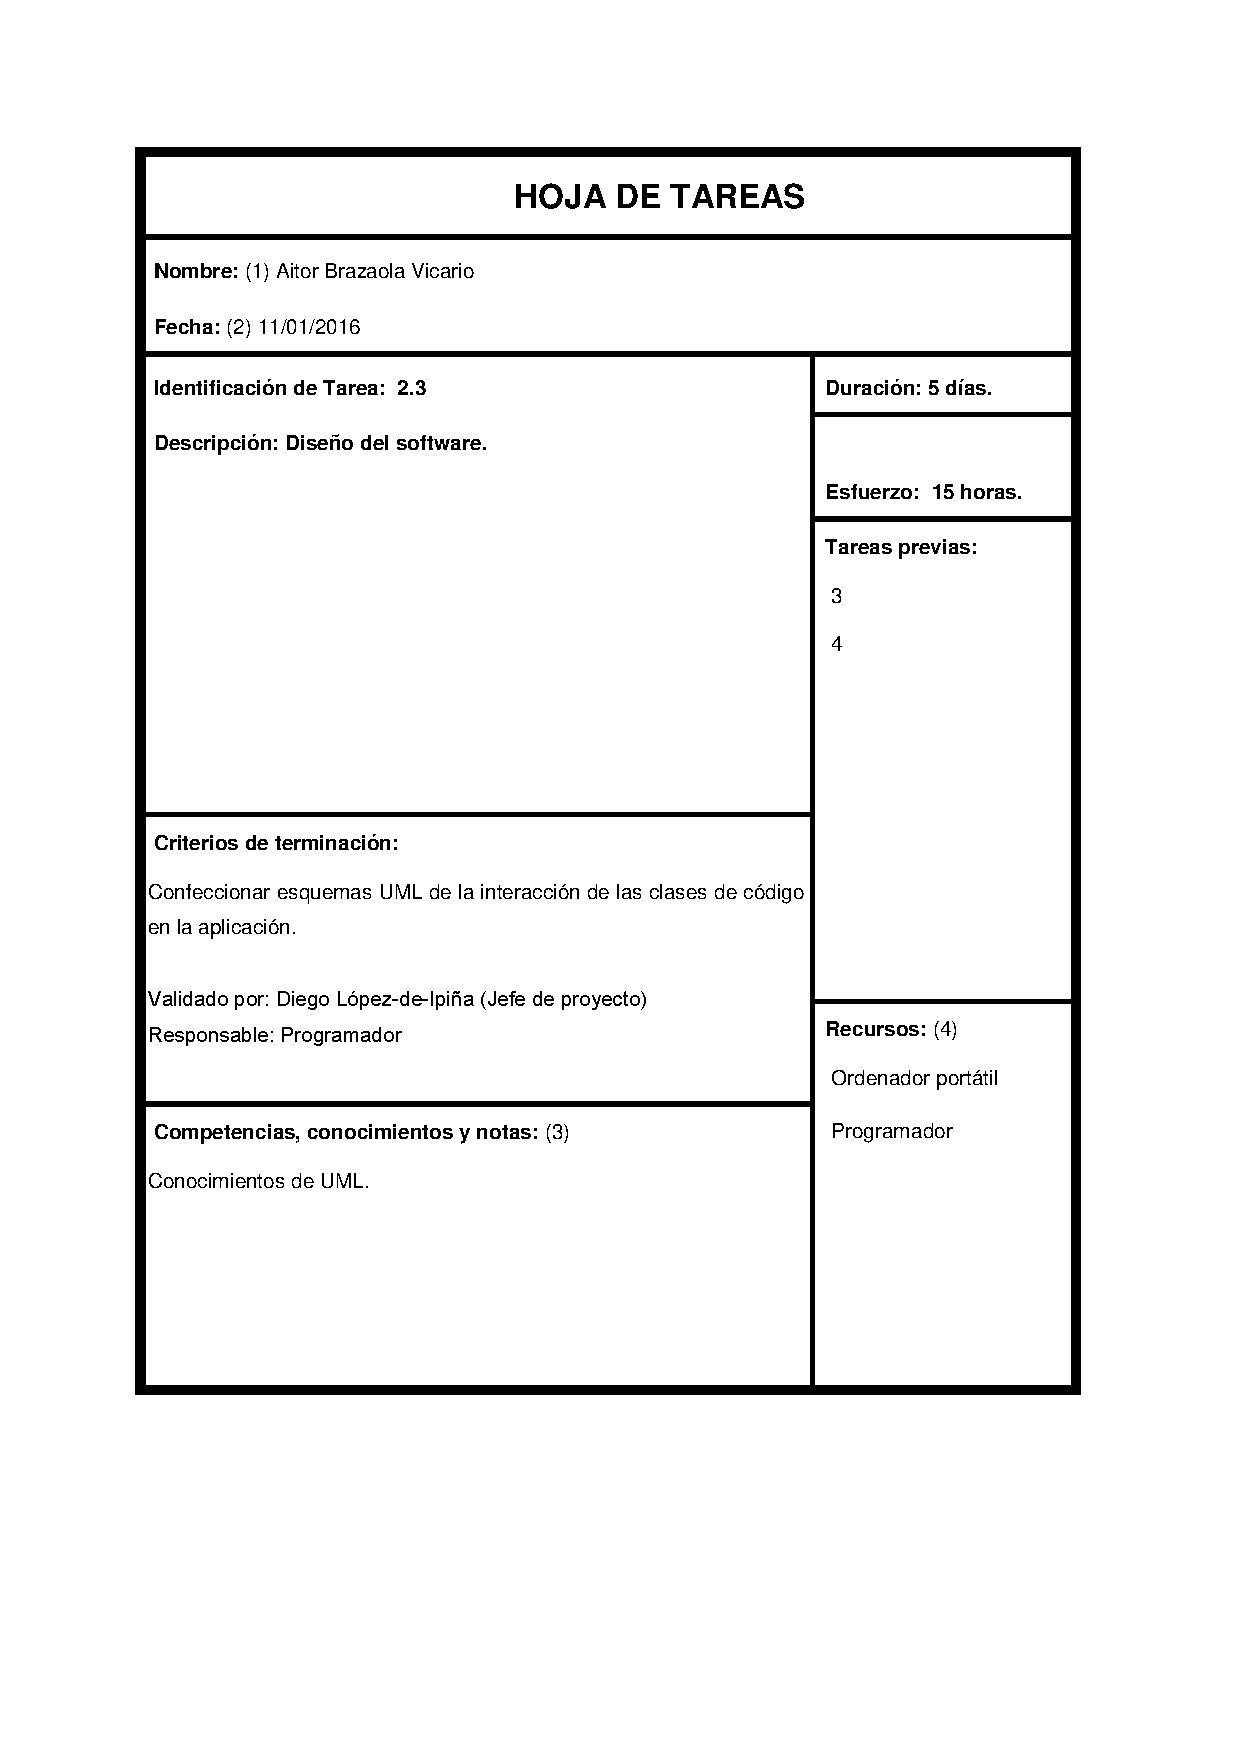
\includegraphics[width=0.9\textwidth]{fig/Tareas/23}
	\caption{Task 2.3.}
	\label{fig:t23}
\end{figure}

\begin{figure}[H]
	\centering
	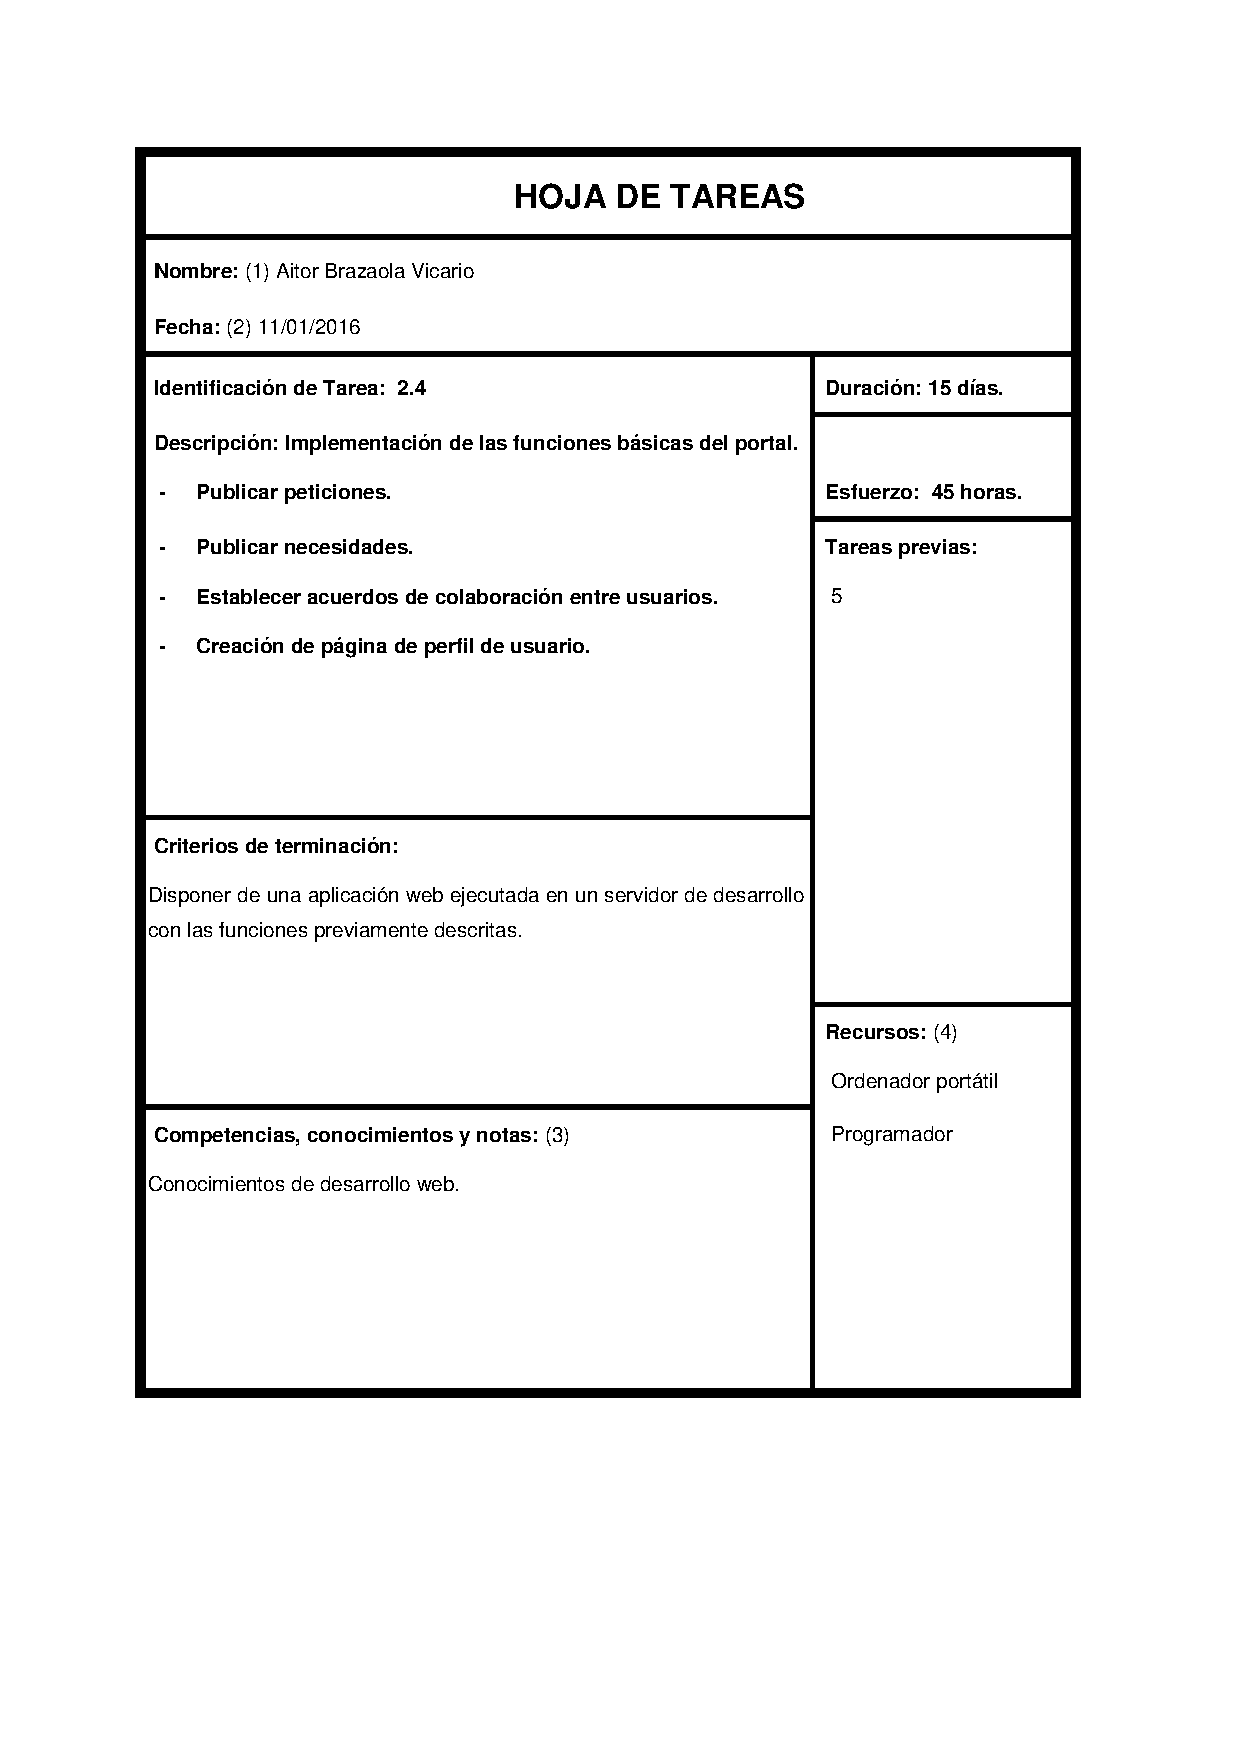
\includegraphics[width=0.9\textwidth]{fig/Tareas/24}
	\caption{Task 2.4.}
	\label{fig:t24}
\end{figure}

\begin{figure}[H]
	\centering
	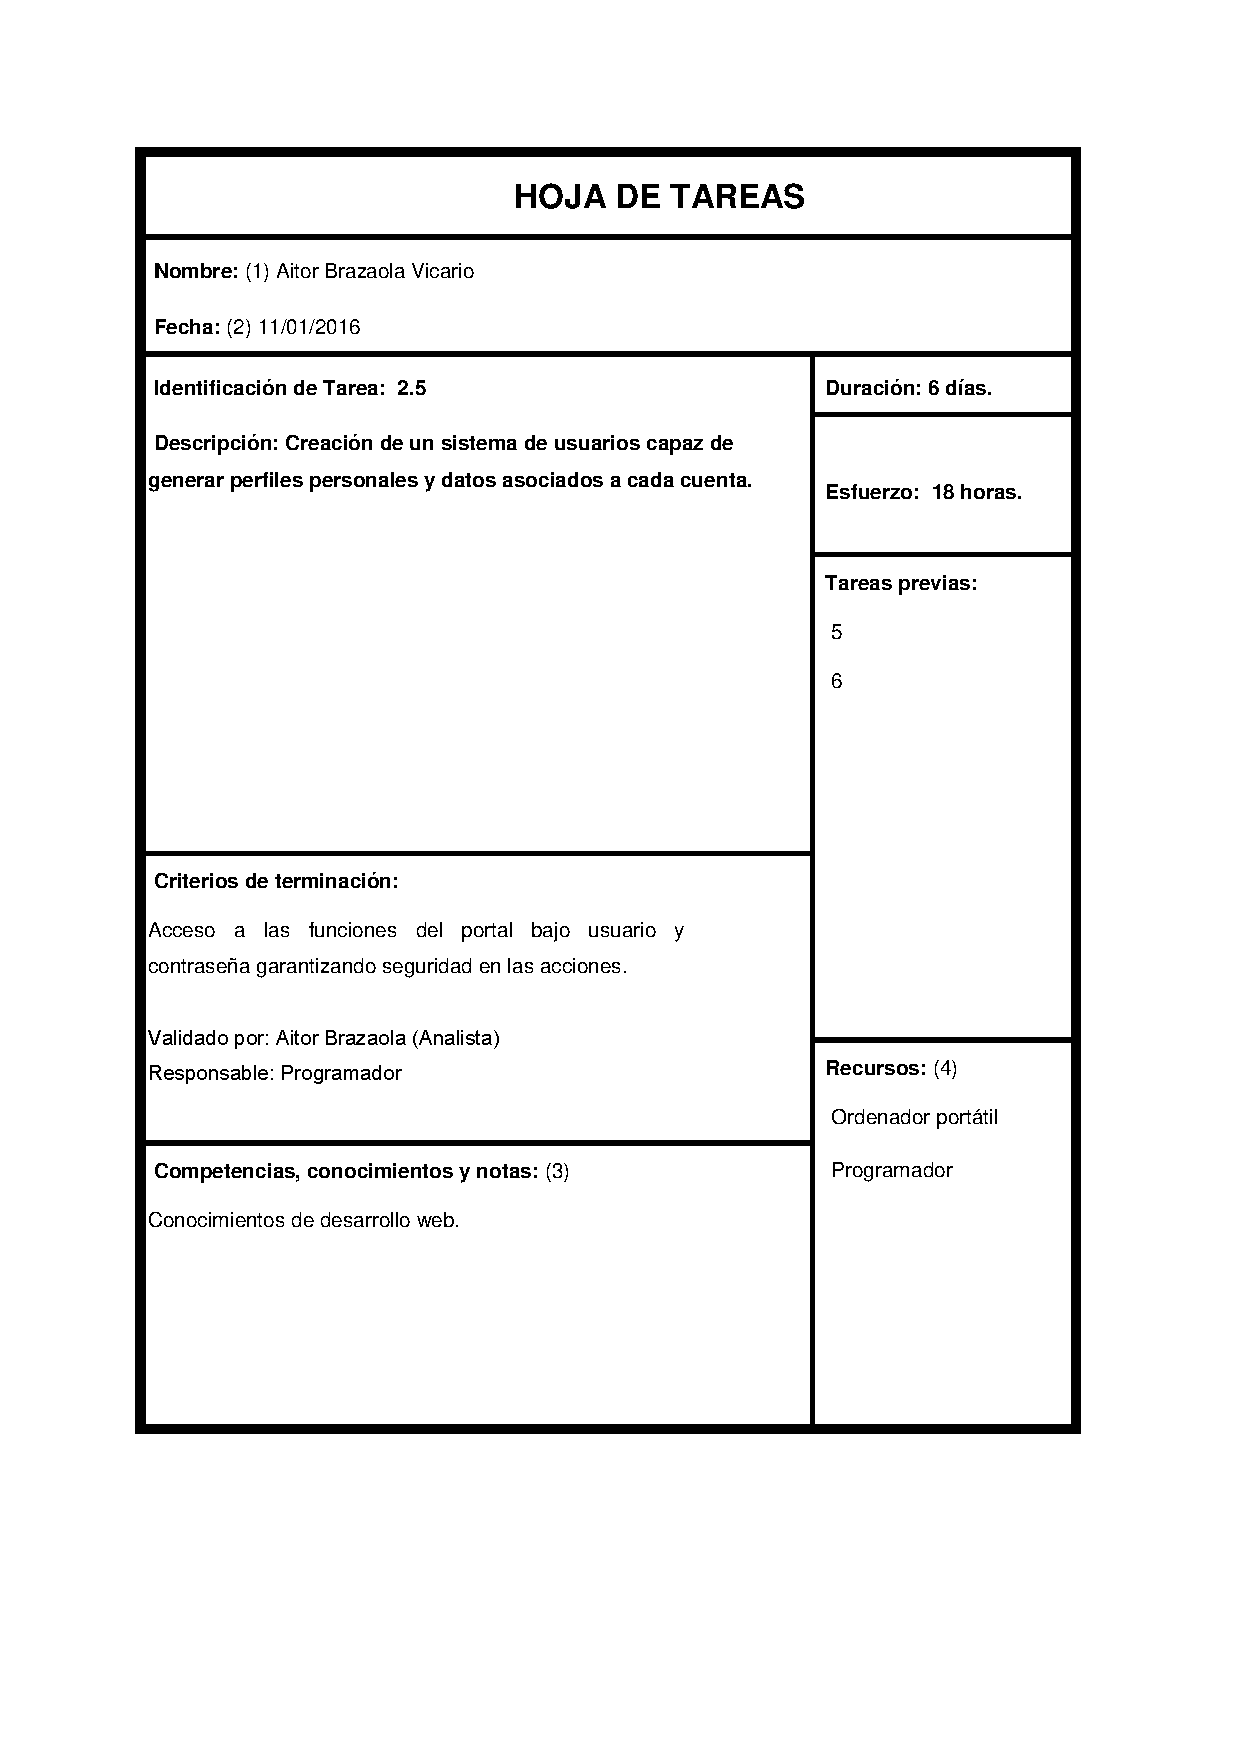
\includegraphics[width=0.9\textwidth]{fig/Tareas/25}
	\caption{Task 2.5.}
	\label{fig:t25}
\end{figure}

\begin{figure}[H]
	\centering
	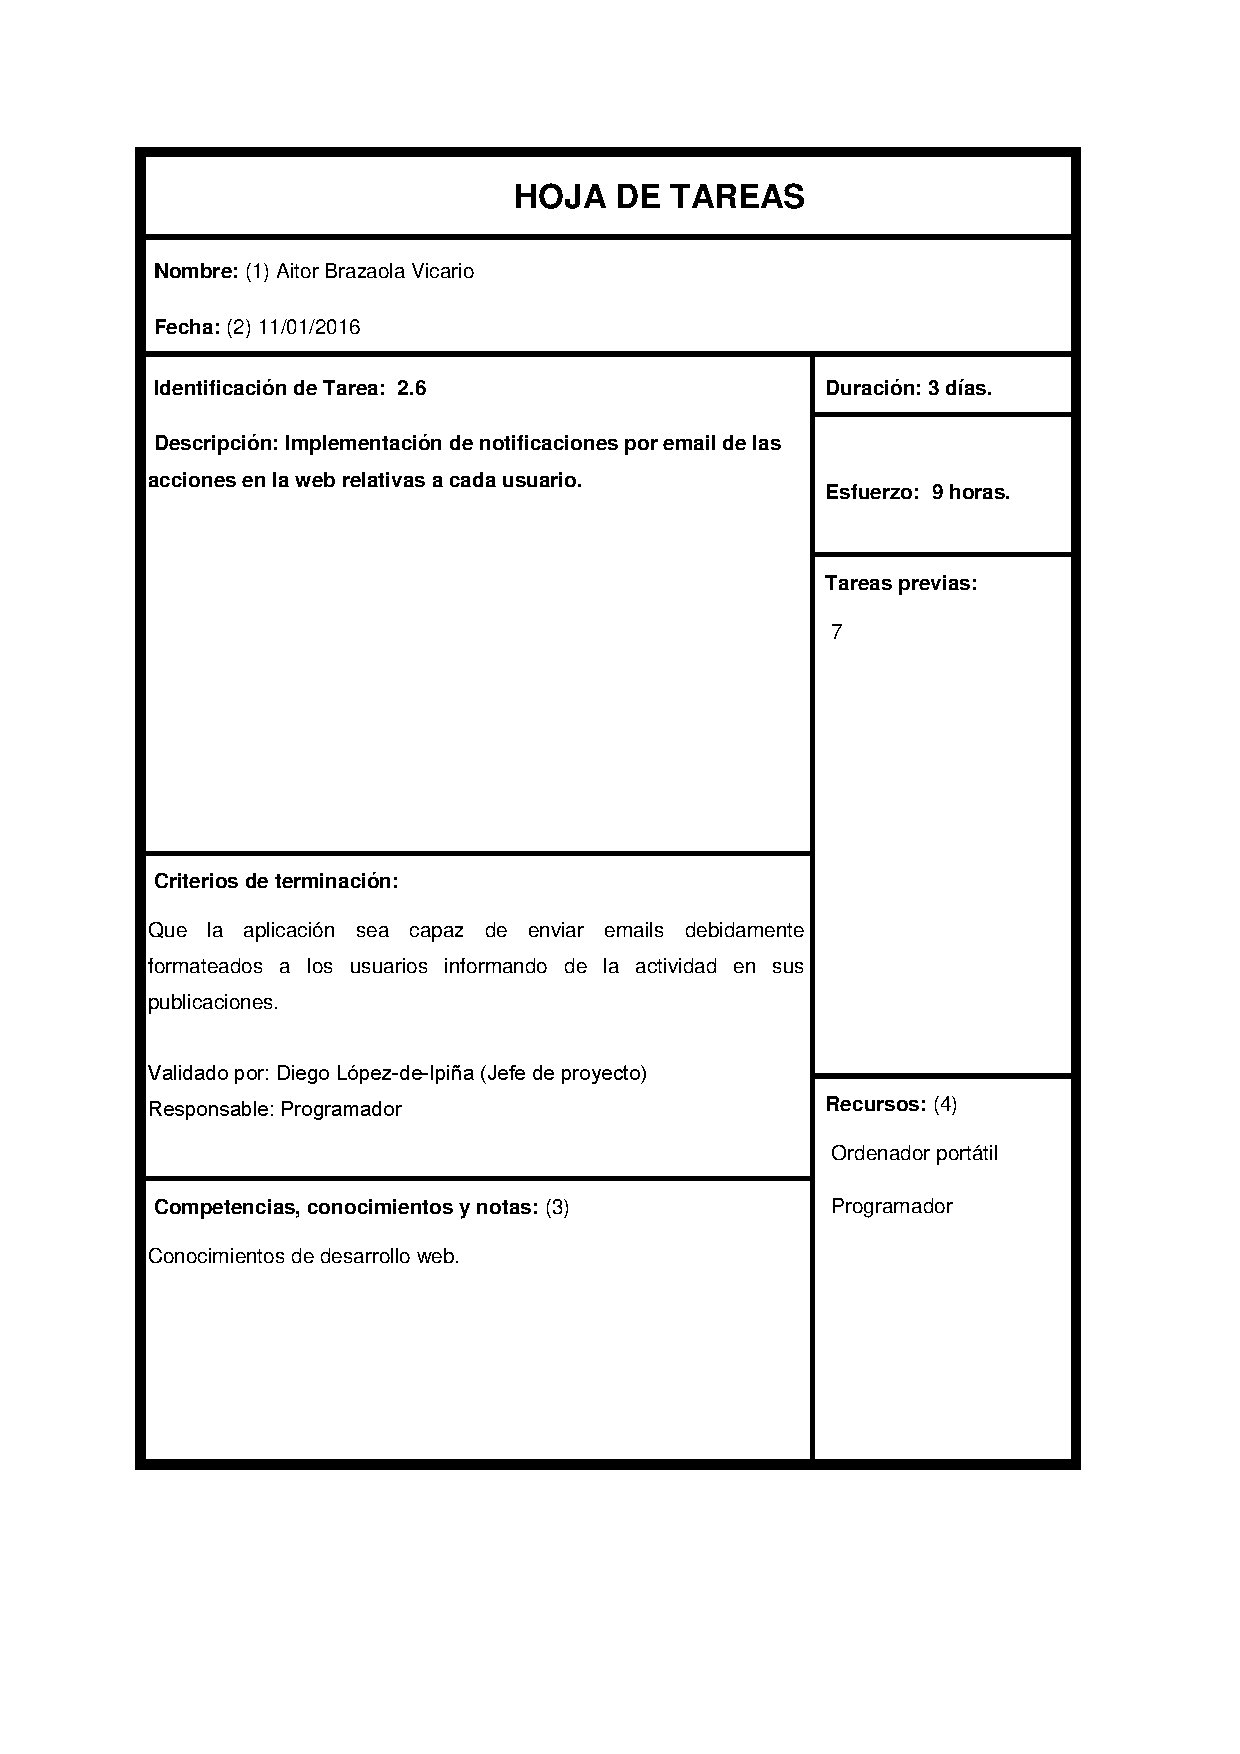
\includegraphics[width=0.9\textwidth]{fig/Tareas/26}
	\caption{Task 2.6.}
	\label{fig:t26}
\end{figure}

\begin{figure}[H]
	\centering
	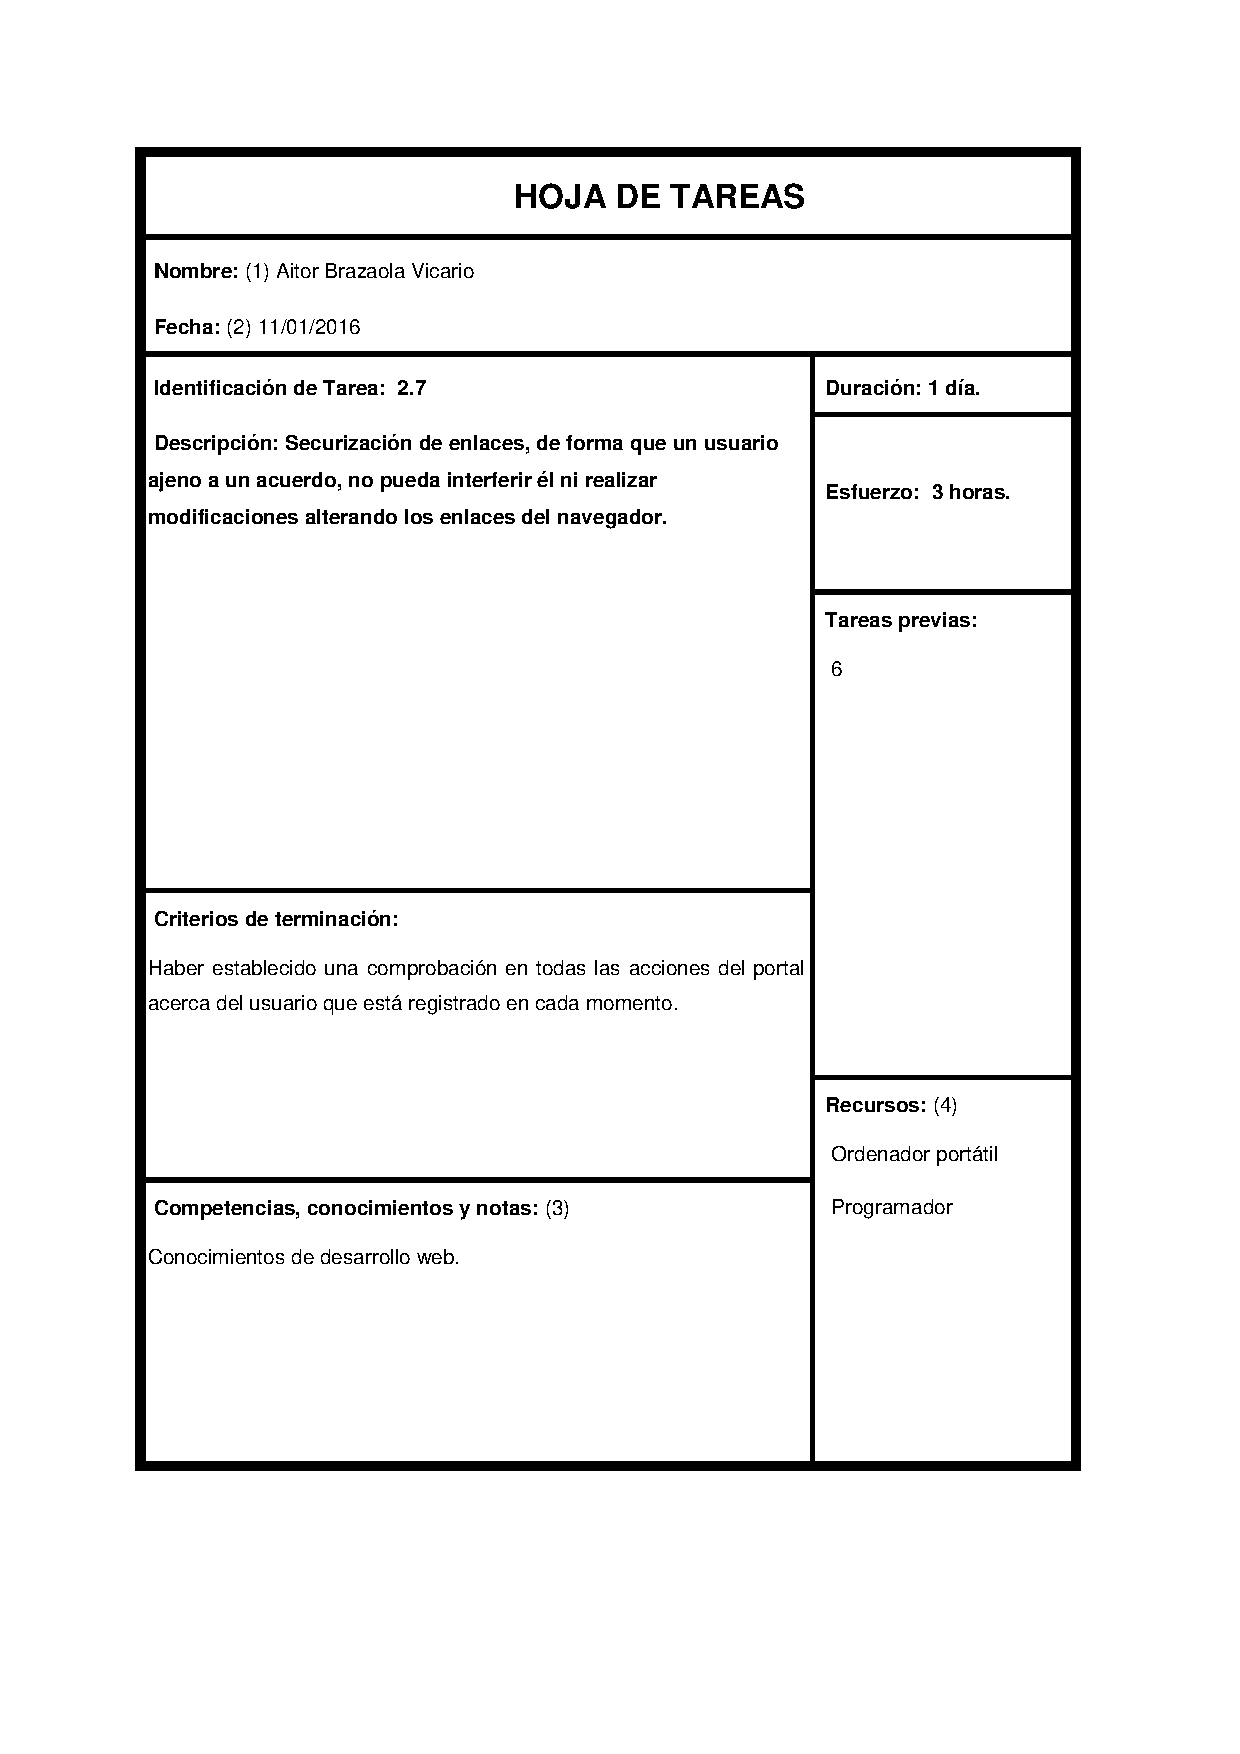
\includegraphics[width=0.9\textwidth]{fig/Tareas/27}
	\caption{Task 2.7.}
	\label{fig:t27}
\end{figure}

\begin{figure}[H]
	\centering
	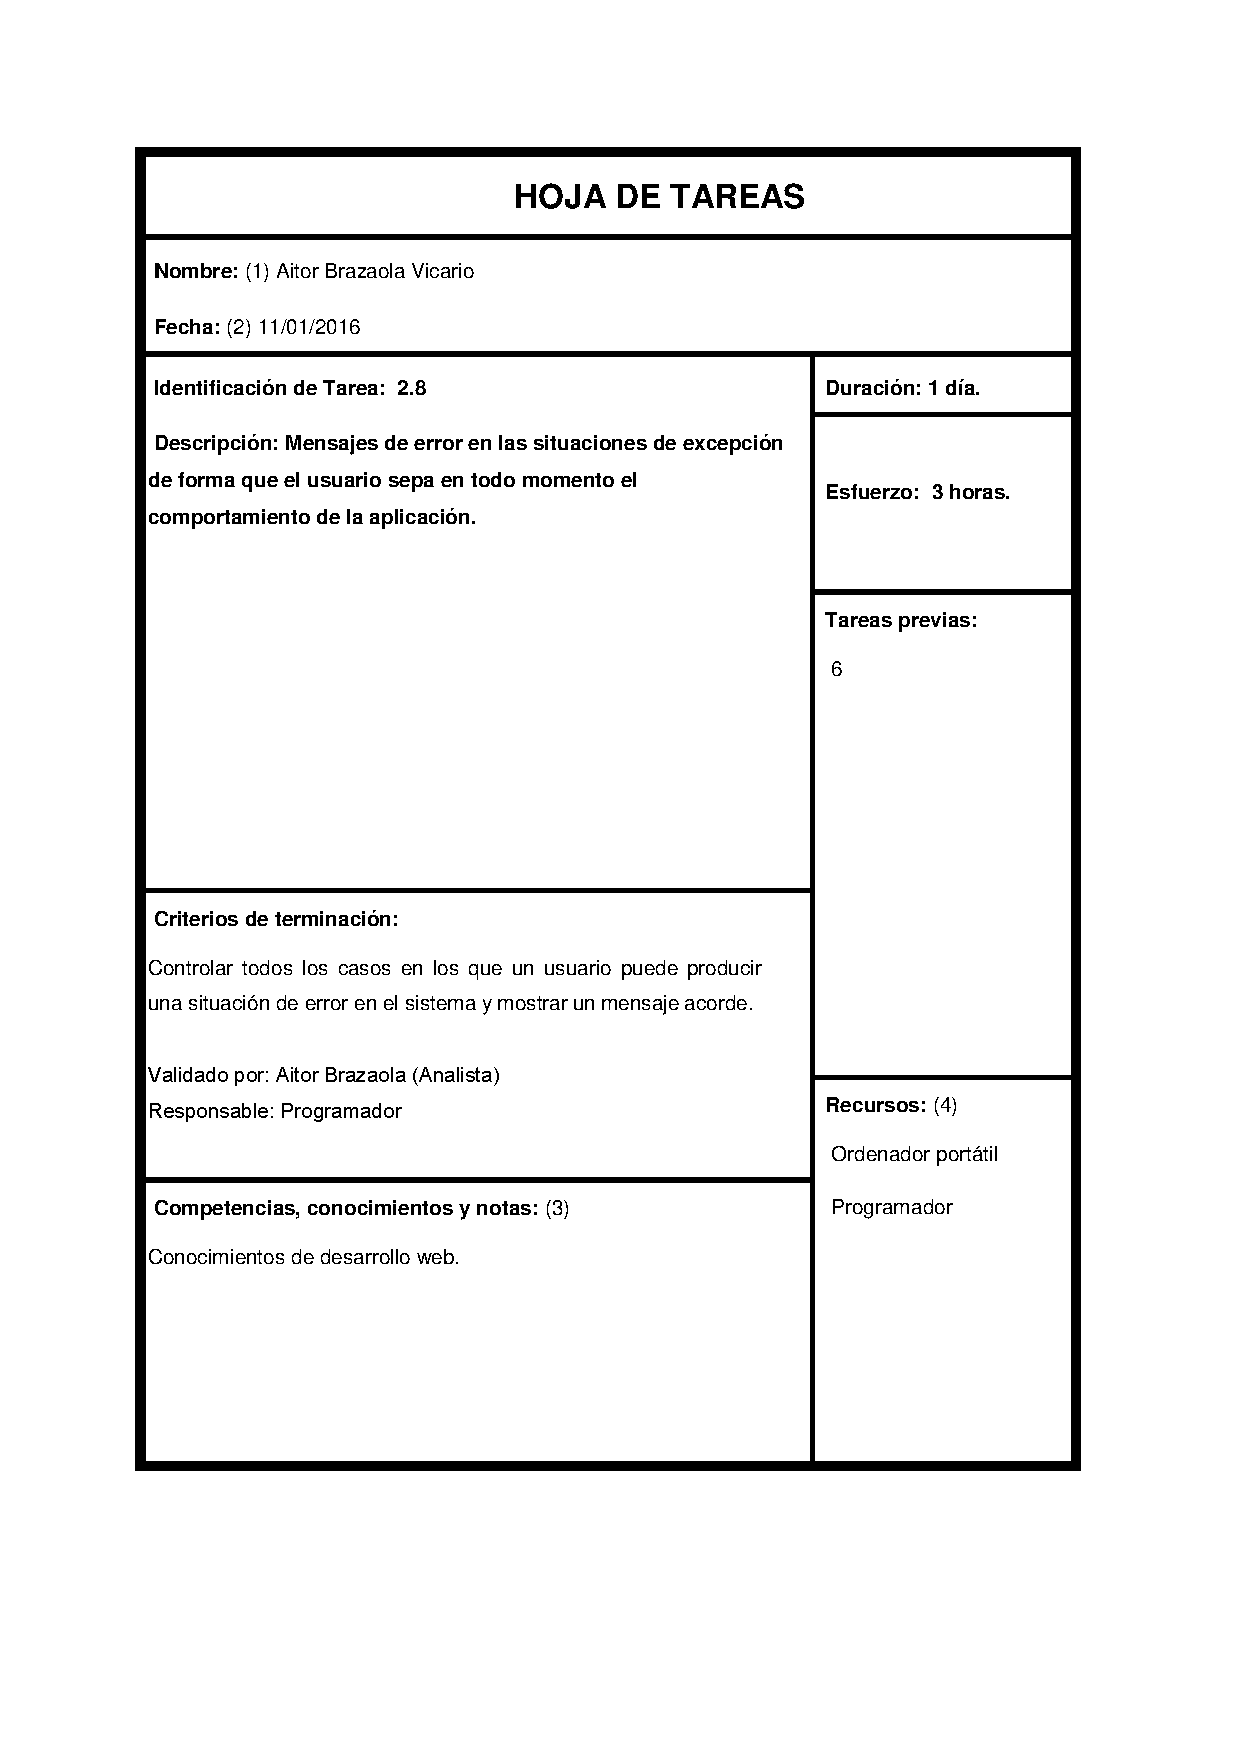
\includegraphics[width=0.9\textwidth]{fig/Tareas/28}
	\caption{Task 2.8.}
	\label{fig:t28}
\end{figure}

\begin{figure}[H]
	\centering
	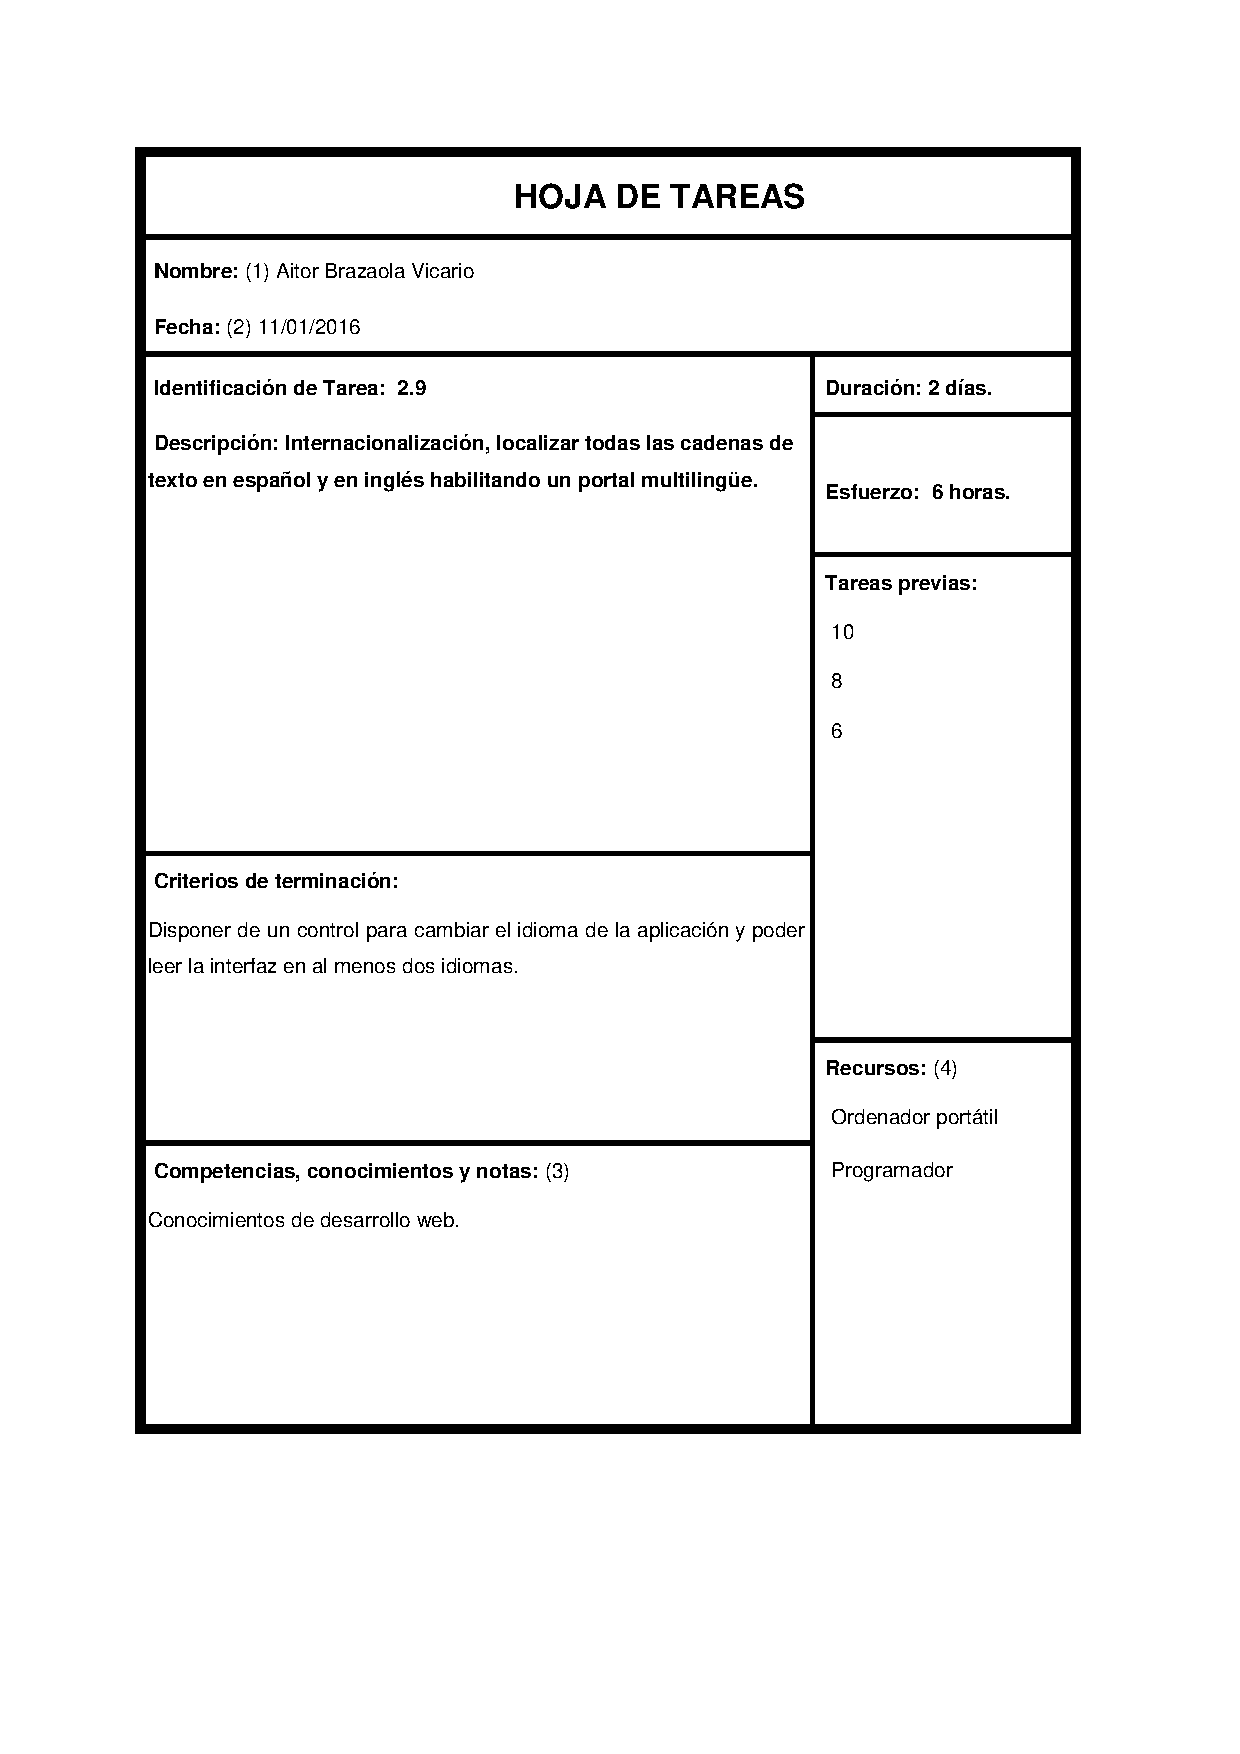
\includegraphics[width=0.9\textwidth]{fig/Tareas/29}
	\caption{Task 2.9.}
	\label{fig:t29}
\end{figure}

\begin{figure}[H]
	\centering
	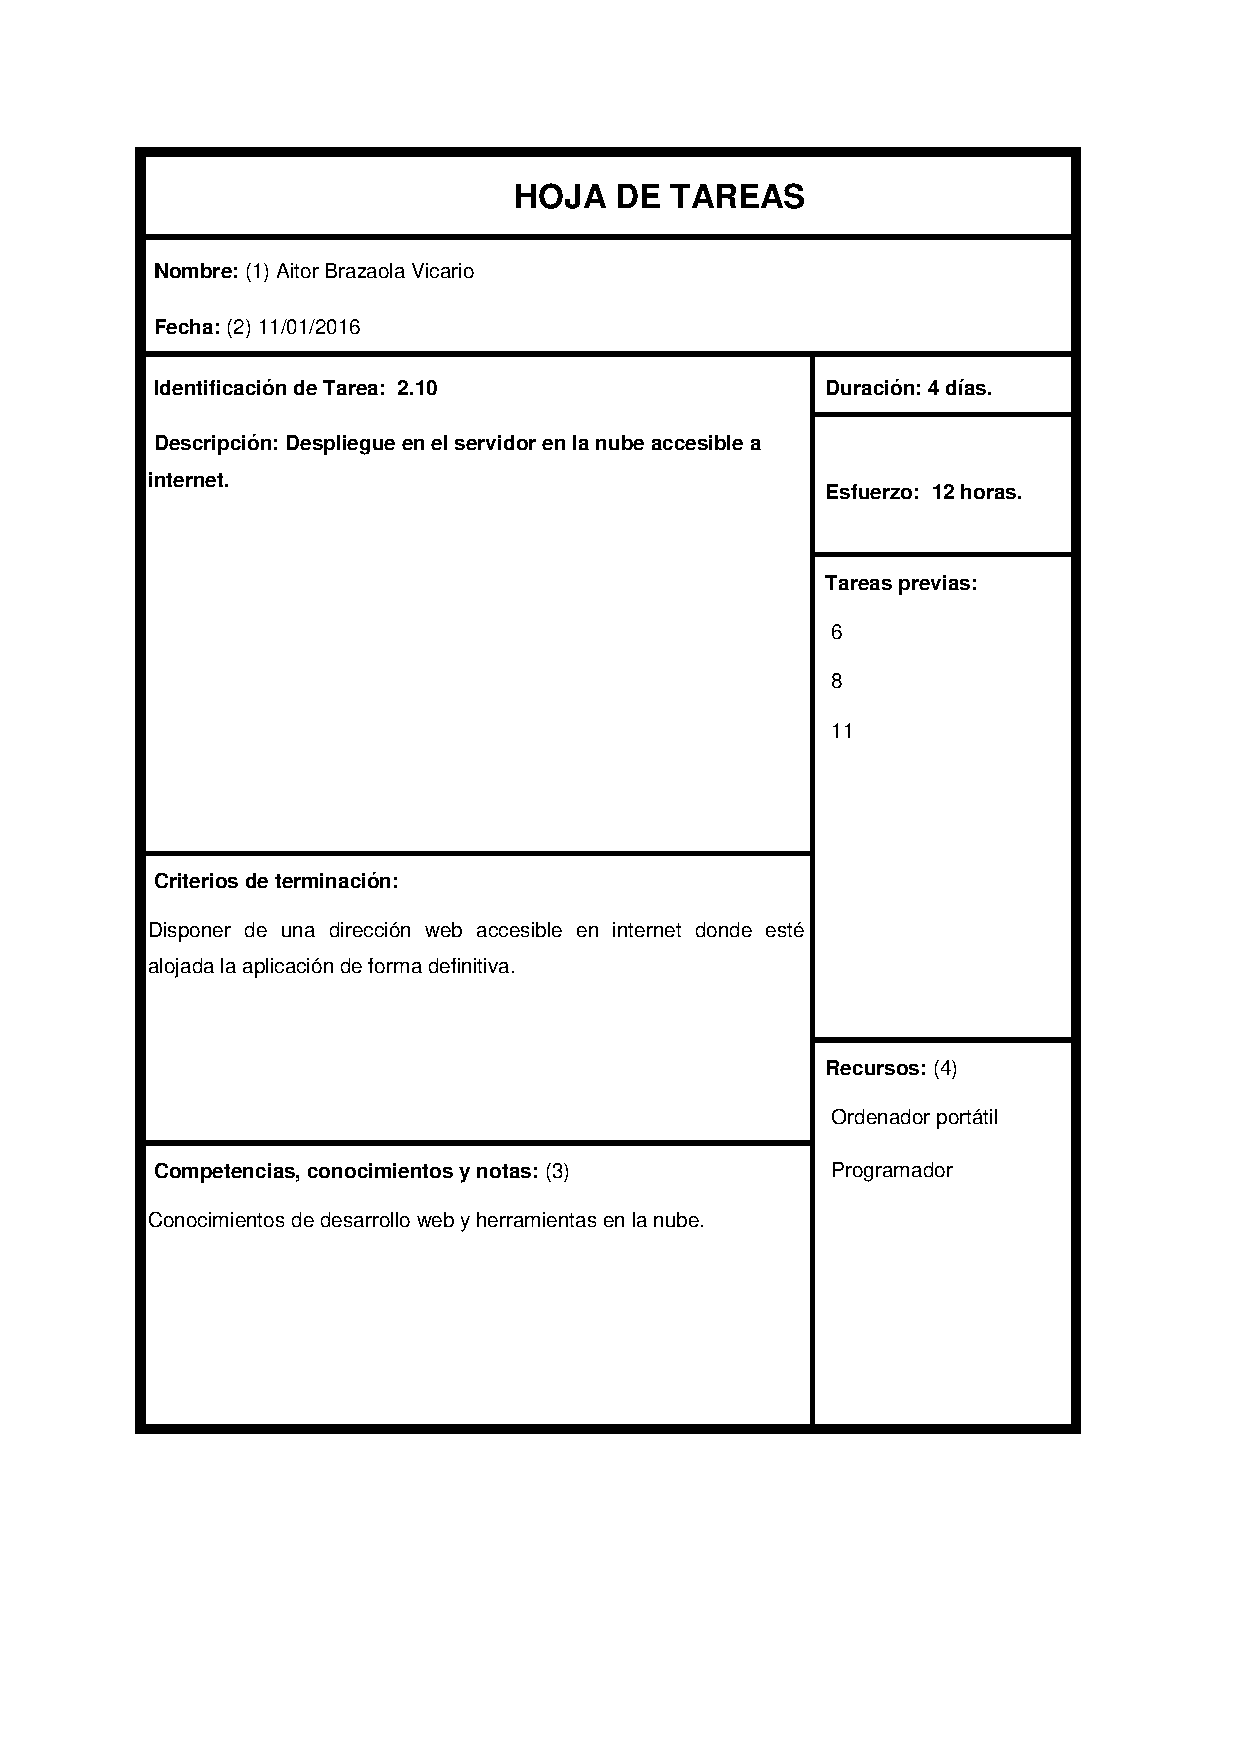
\includegraphics[width=0.9\textwidth]{fig/Tareas/210}
	\caption{Task 2.10.}
	\label{fig:t210}
\end{figure}

\begin{figure}[H]
	\centering
	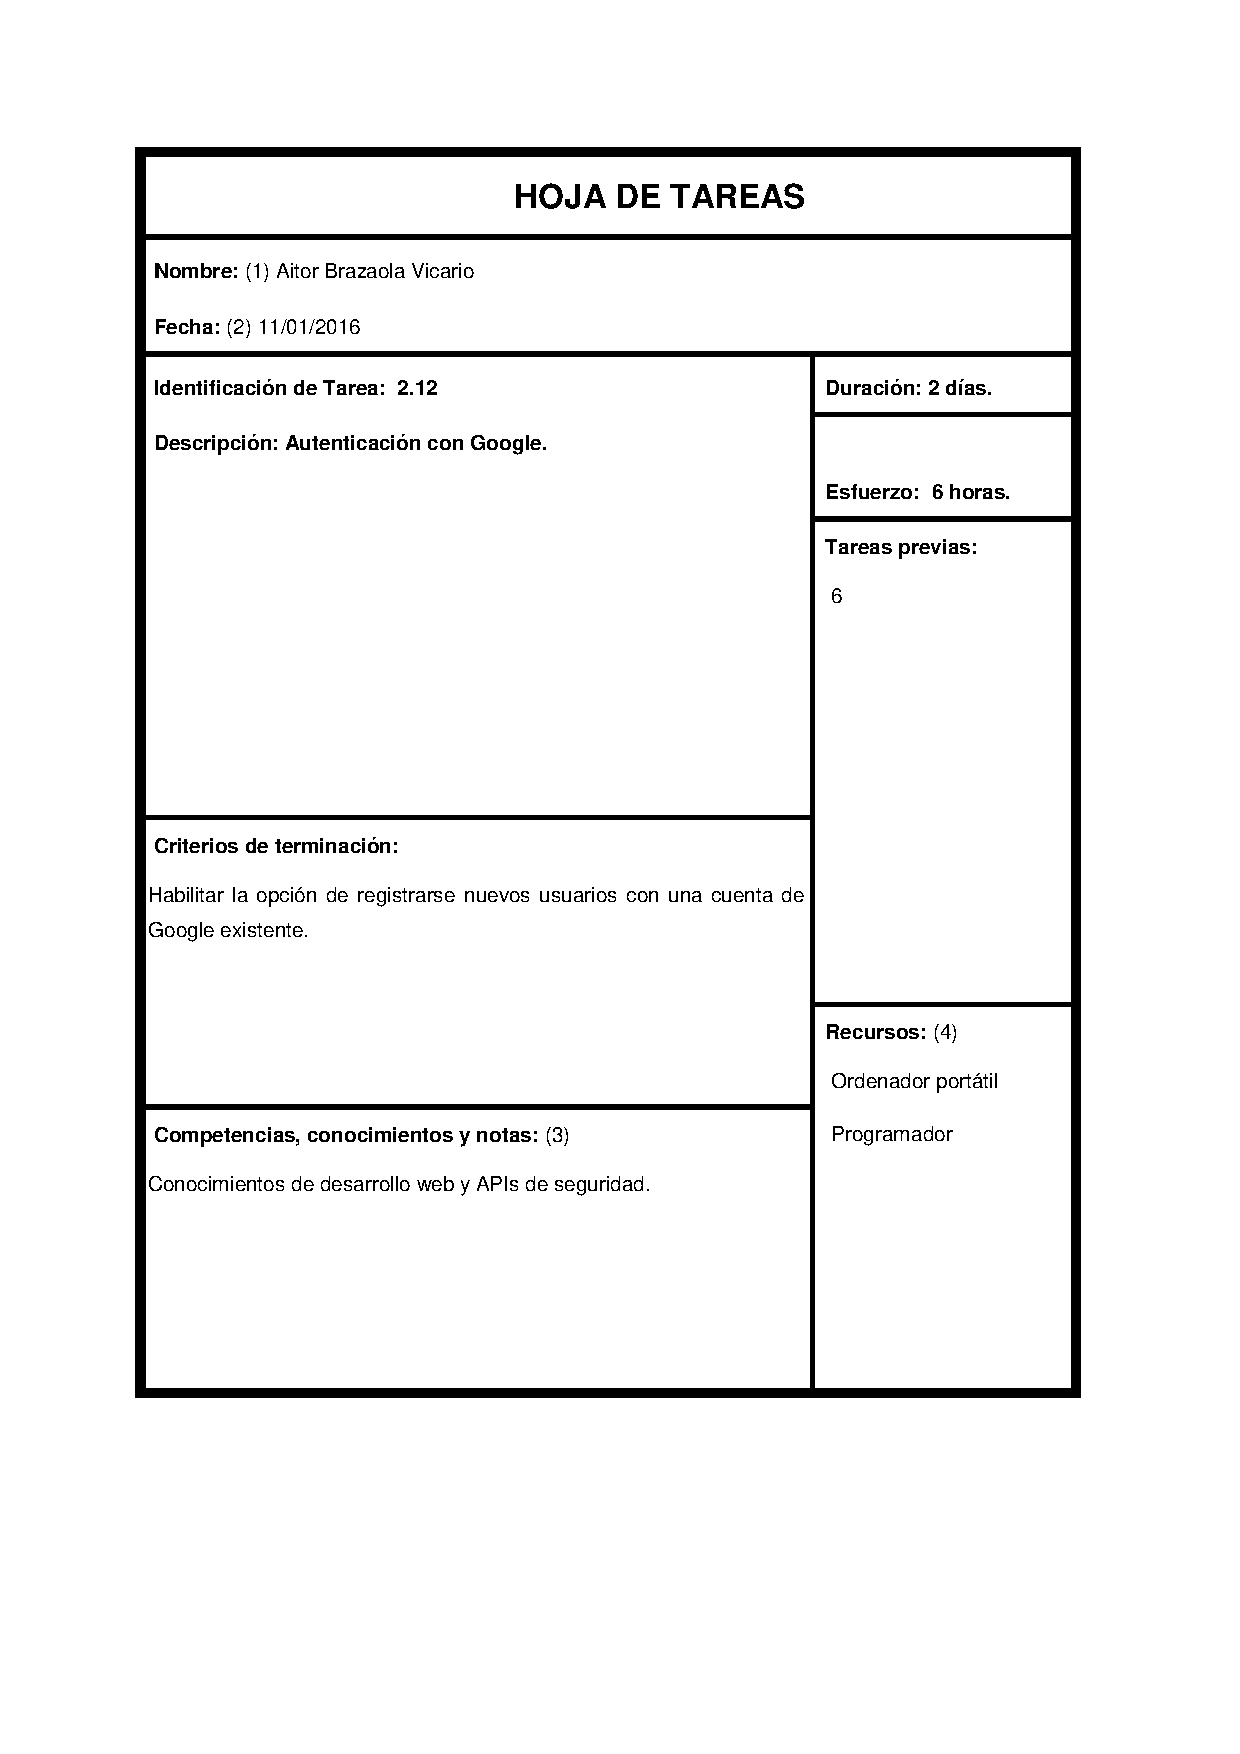
\includegraphics[width=0.9\textwidth]{fig/Tareas/212}
	\caption{Task 2.12.}
	\label{fig:t212}
\end{figure}

\begin{figure}[H]
	\centering
	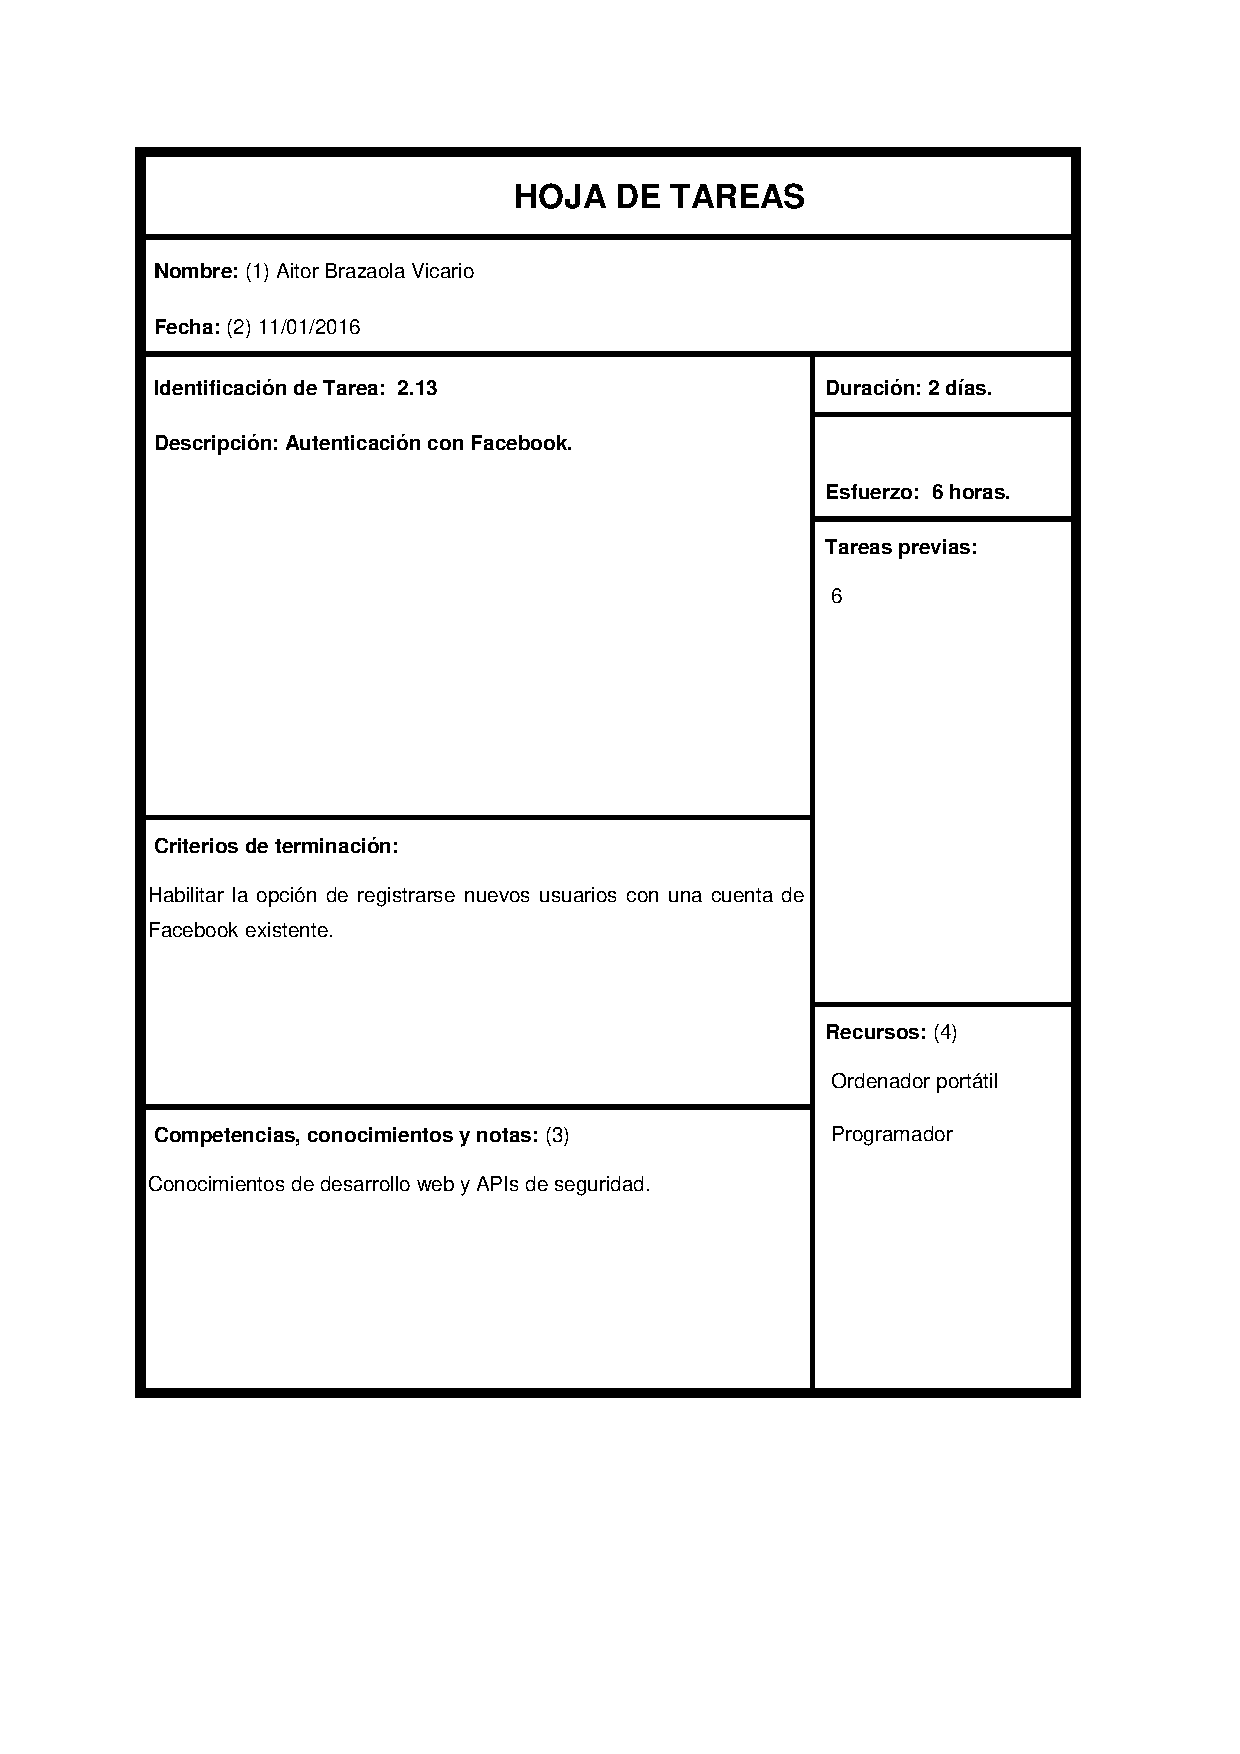
\includegraphics[width=0.9\textwidth]{fig/Tareas/213}
	\caption{Task 2.13.}
	\label{fig:t213}
\end{figure}

\begin{figure}[H]
	\centering
	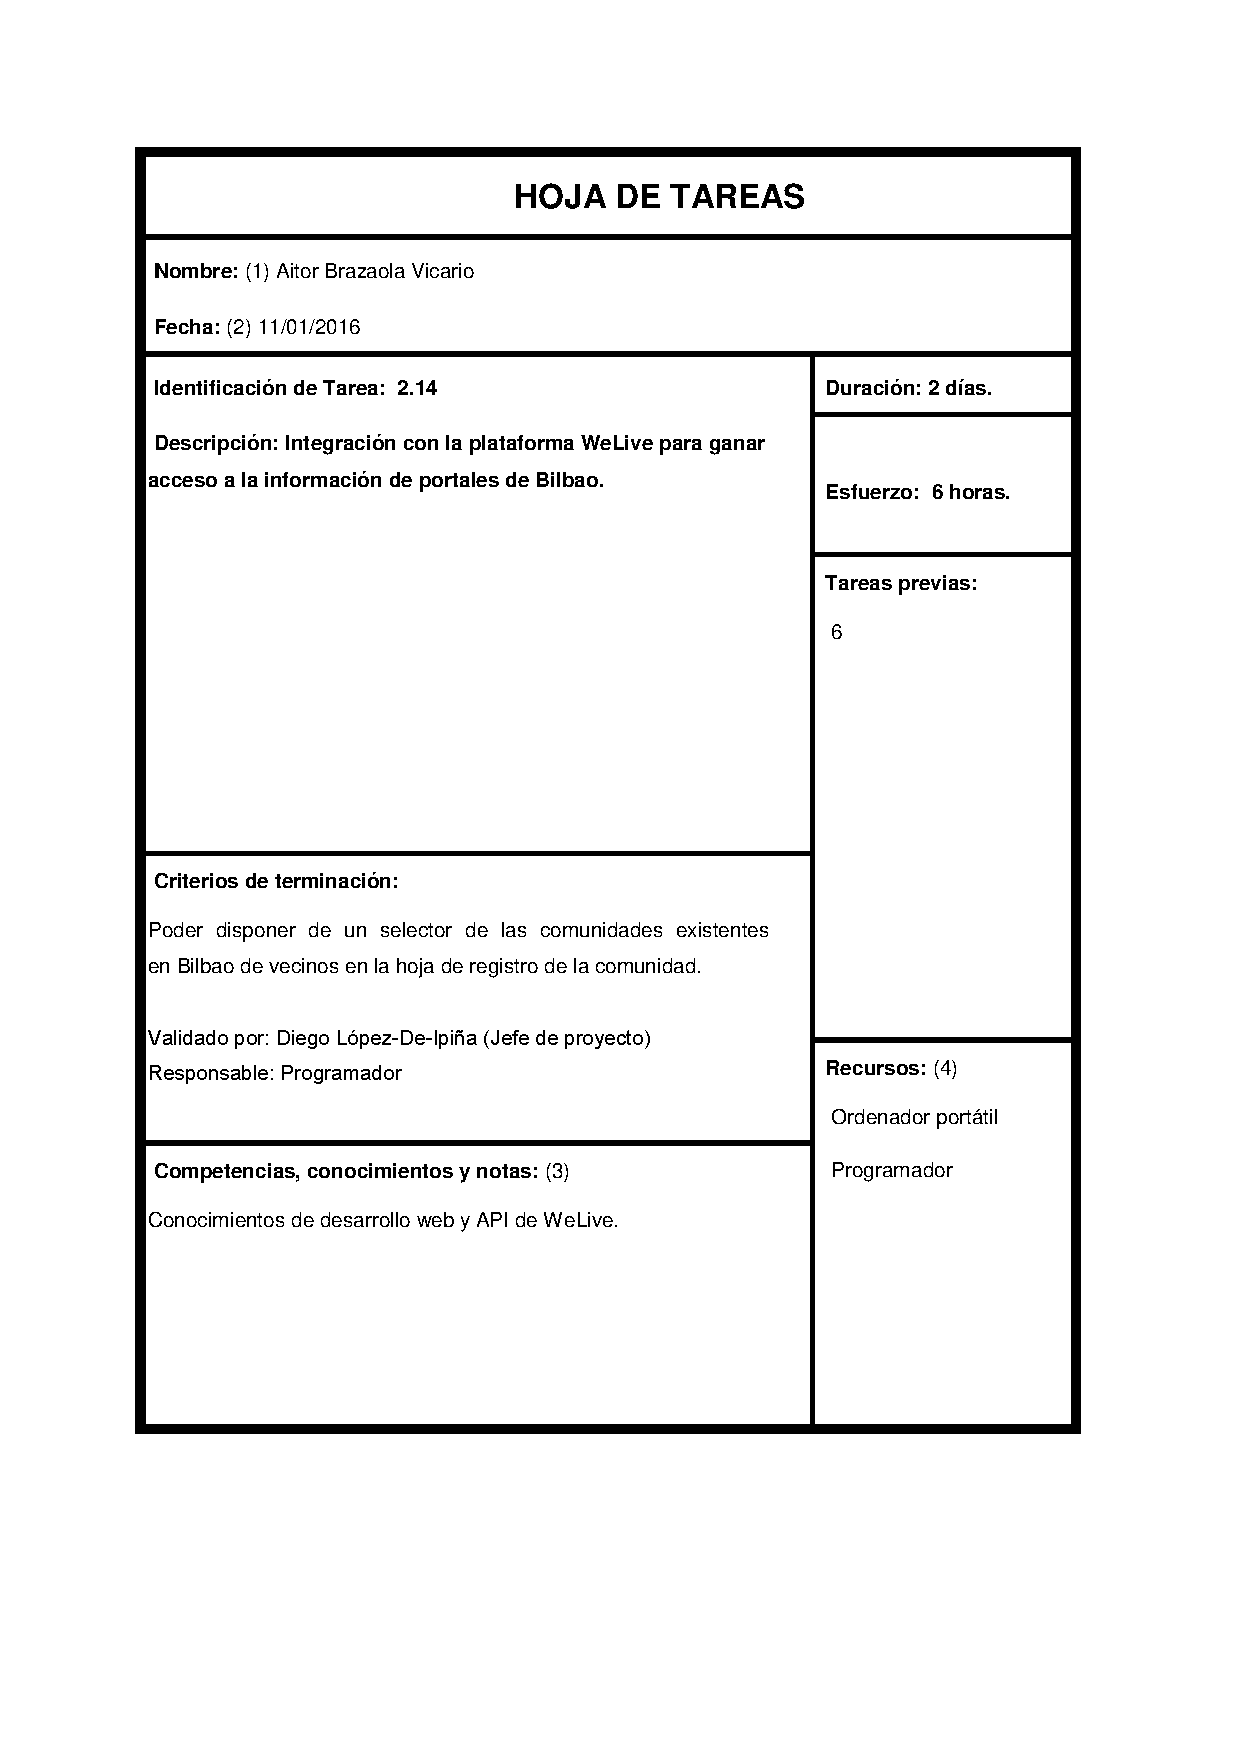
\includegraphics[width=0.9\textwidth]{fig/Tareas/214}
	\caption{Task 2.14.}
	\label{fig:t214}
\end{figure}

\begin{figure}[H]
	\centering
	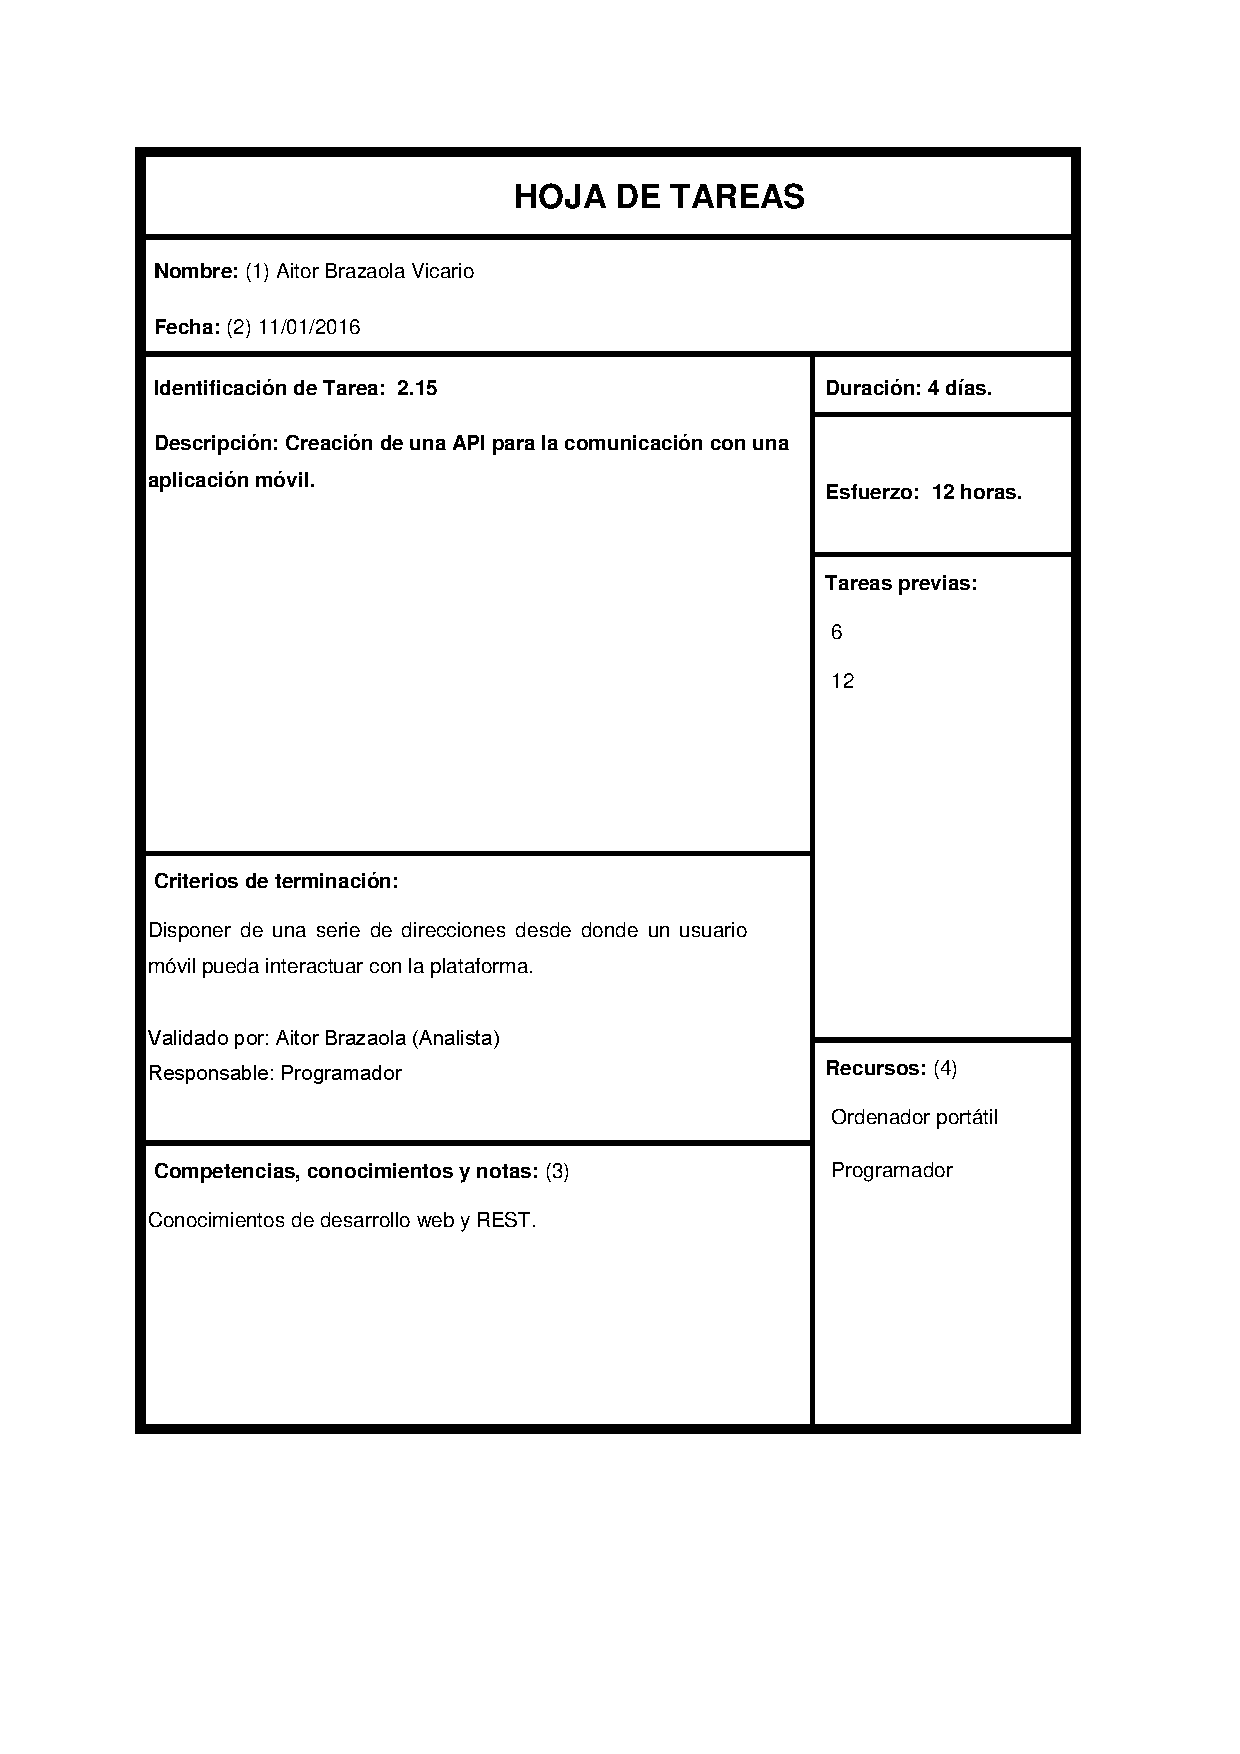
\includegraphics[width=0.9\textwidth]{fig/Tareas/215}
	\caption{Task 2.15.}
	\label{fig:t215}
\end{figure}

\begin{figure}[H]
	\centering
	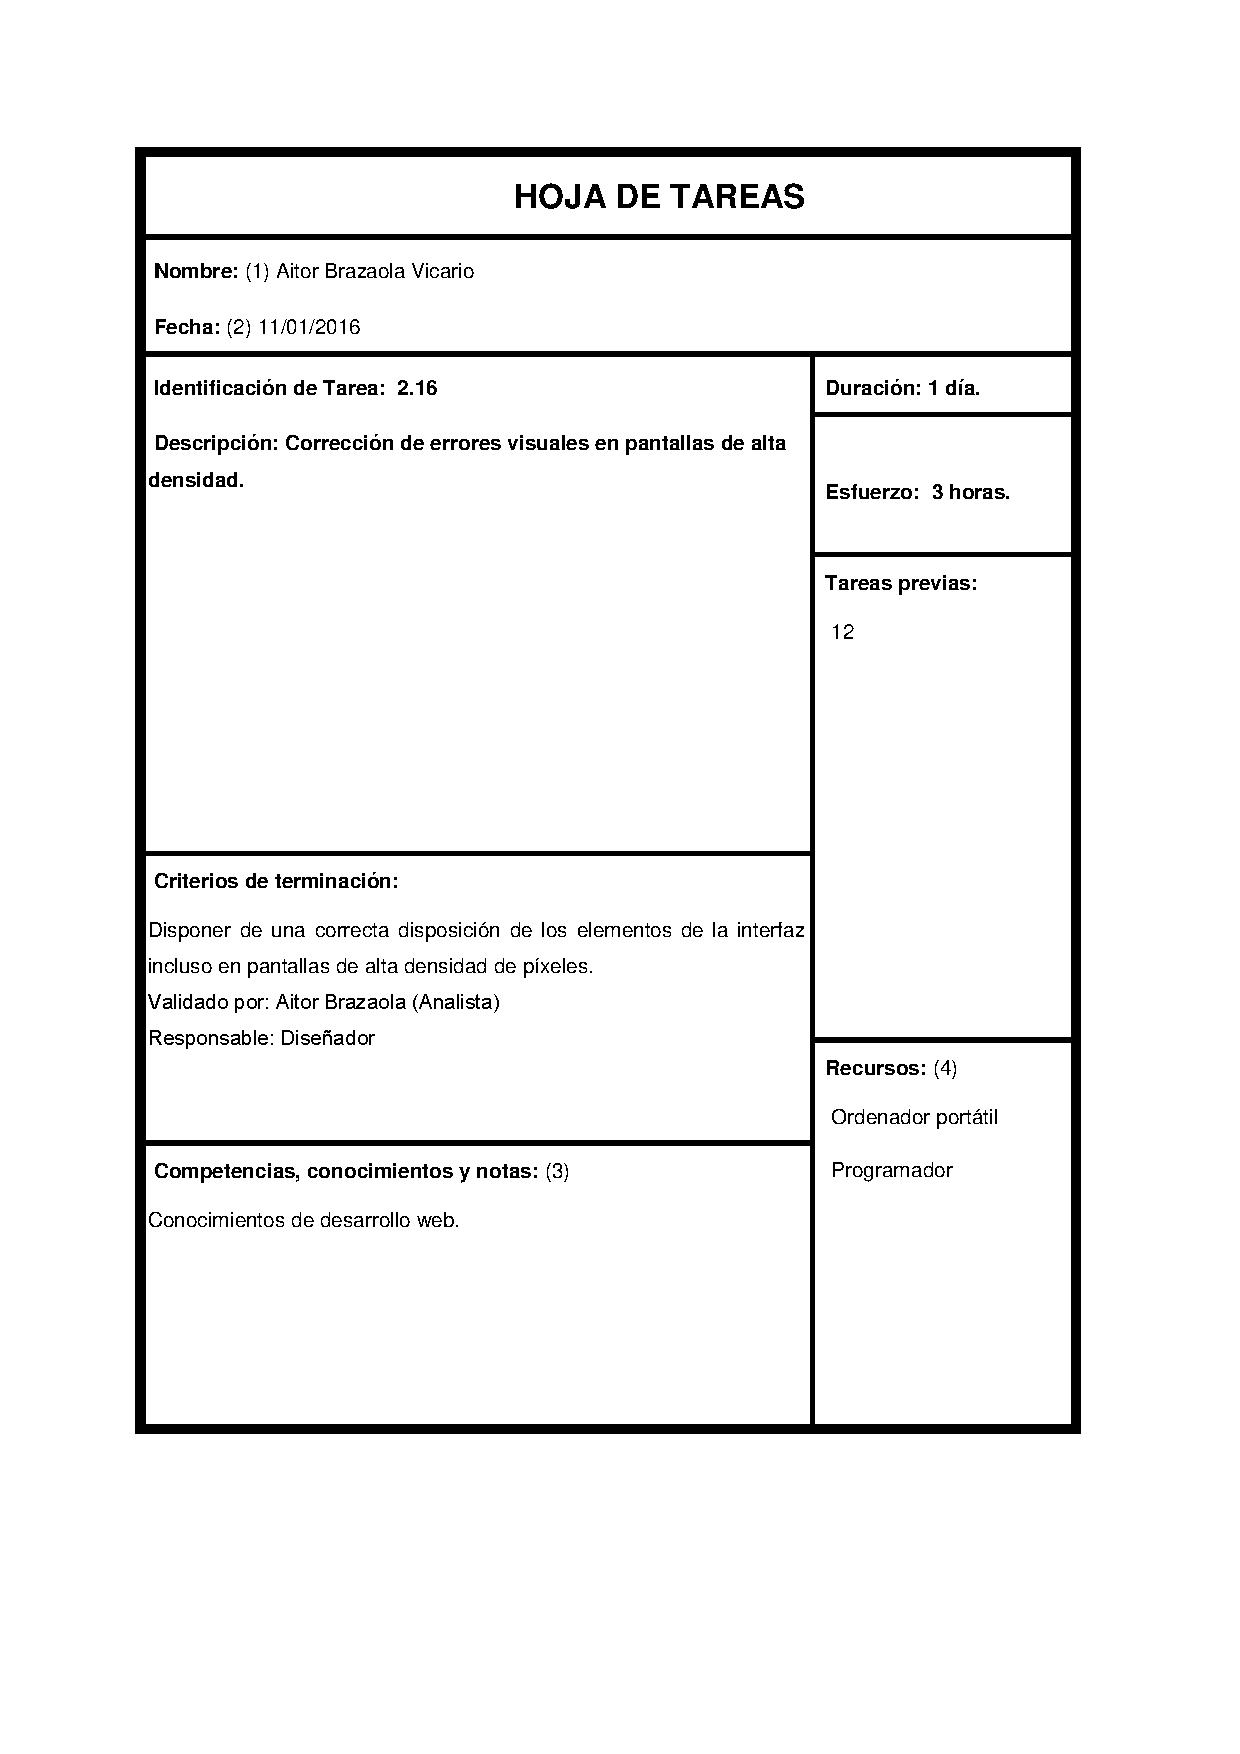
\includegraphics[width=0.9\textwidth]{fig/Tareas/216}
	\caption{Task 2.16.}
	\label{fig:t216}
\end{figure}

\begin{figure}[H]
	\centering
	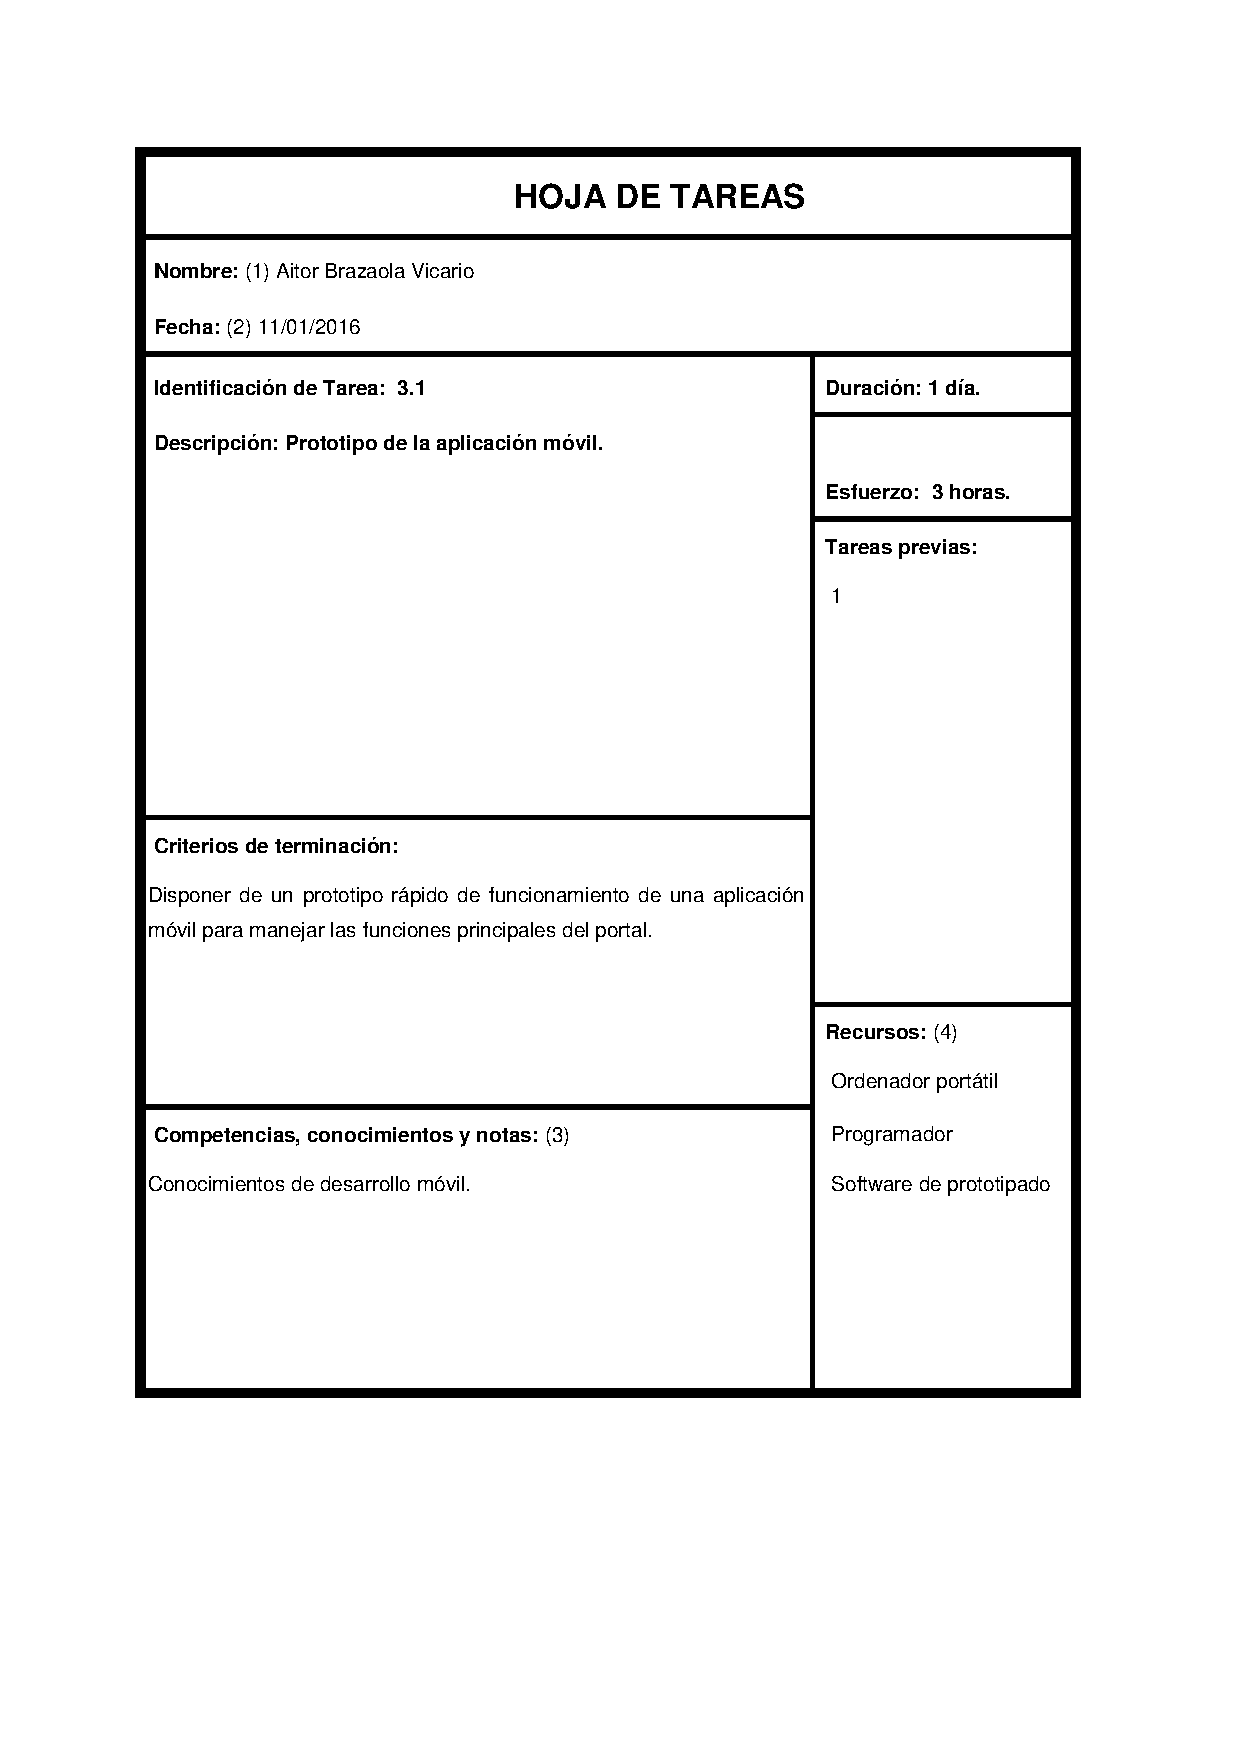
\includegraphics[width=0.9\textwidth]{fig/Tareas/31}
	\caption{Task 3.1.}
	\label{fig:t31}
\end{figure}

\begin{figure}[H]
	\centering
	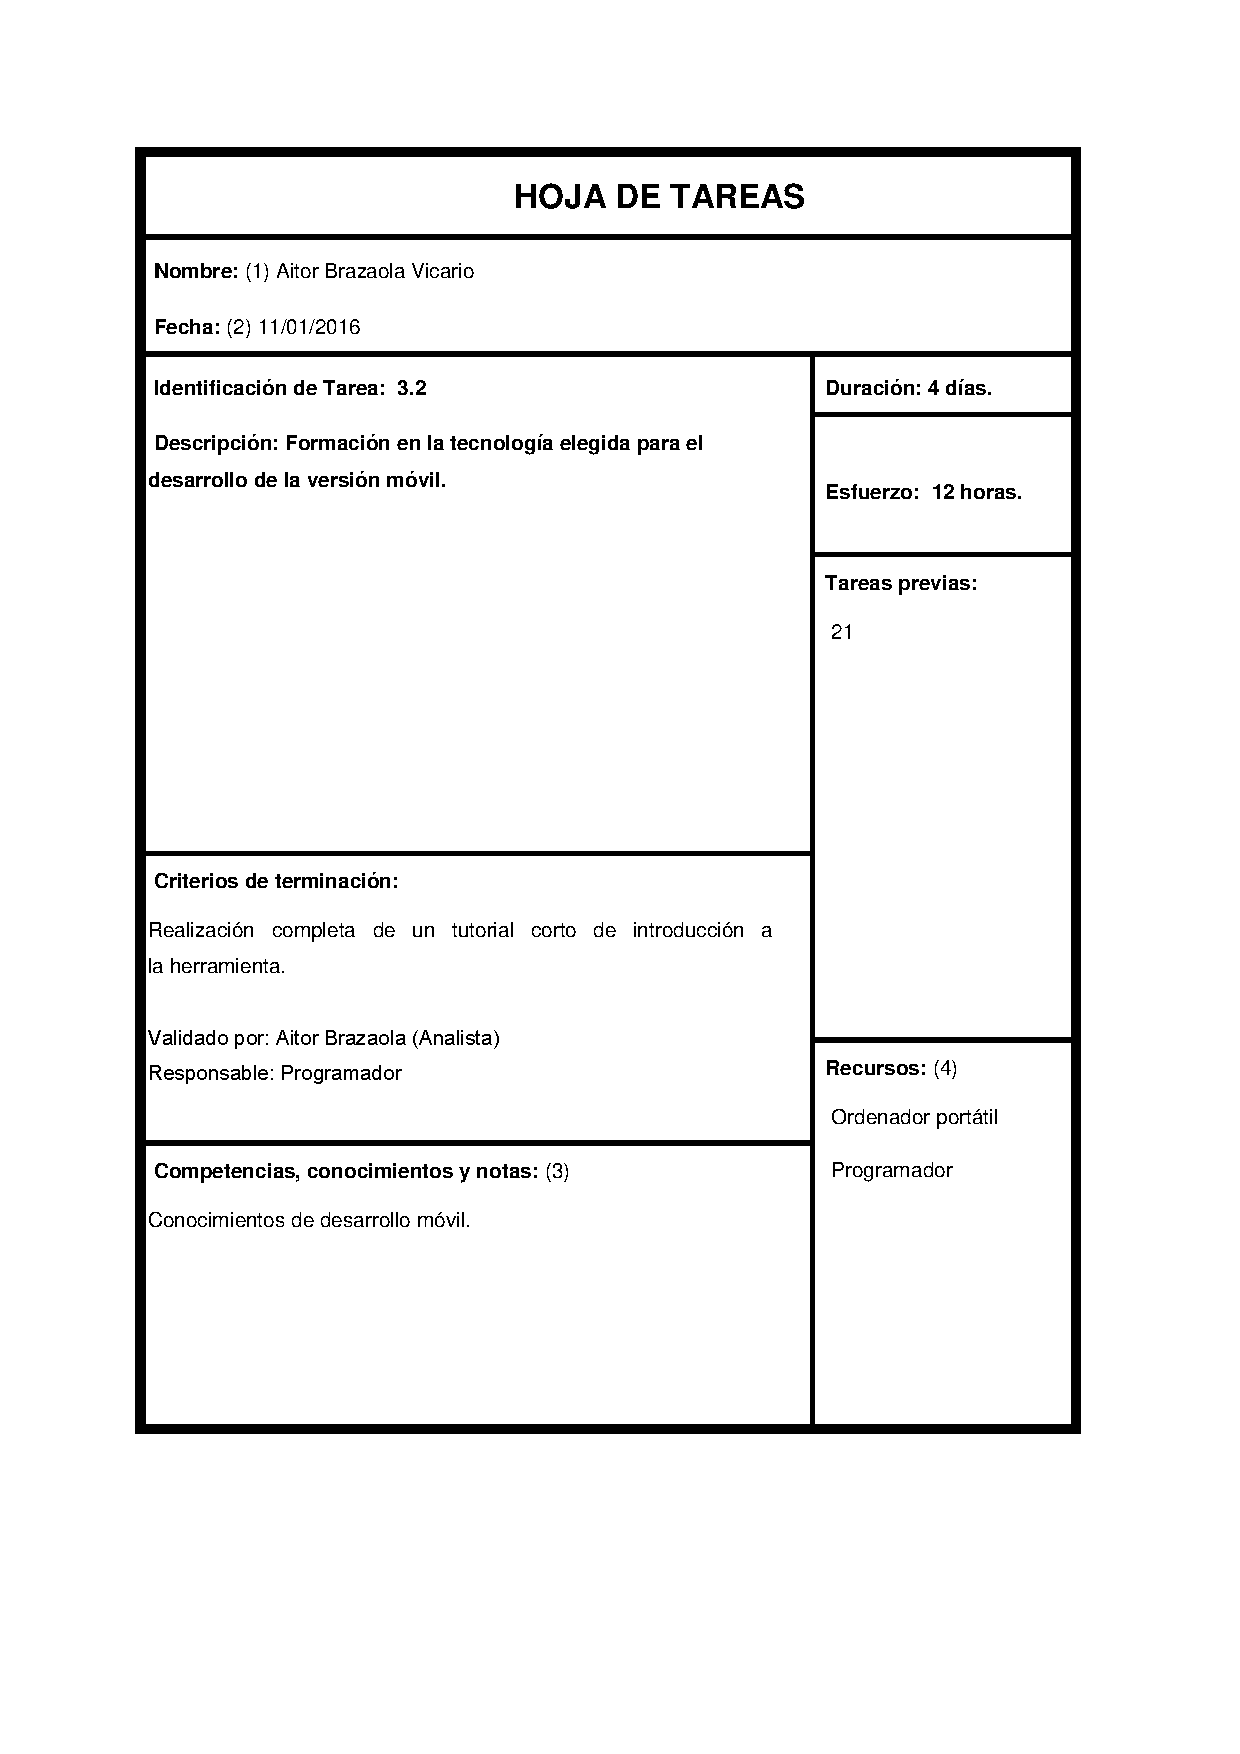
\includegraphics[width=0.9\textwidth]{fig/Tareas/32}
	\caption{Task 3.2.}
	\label{fig:t32}
\end{figure}

\begin{figure}[H]
	\centering
	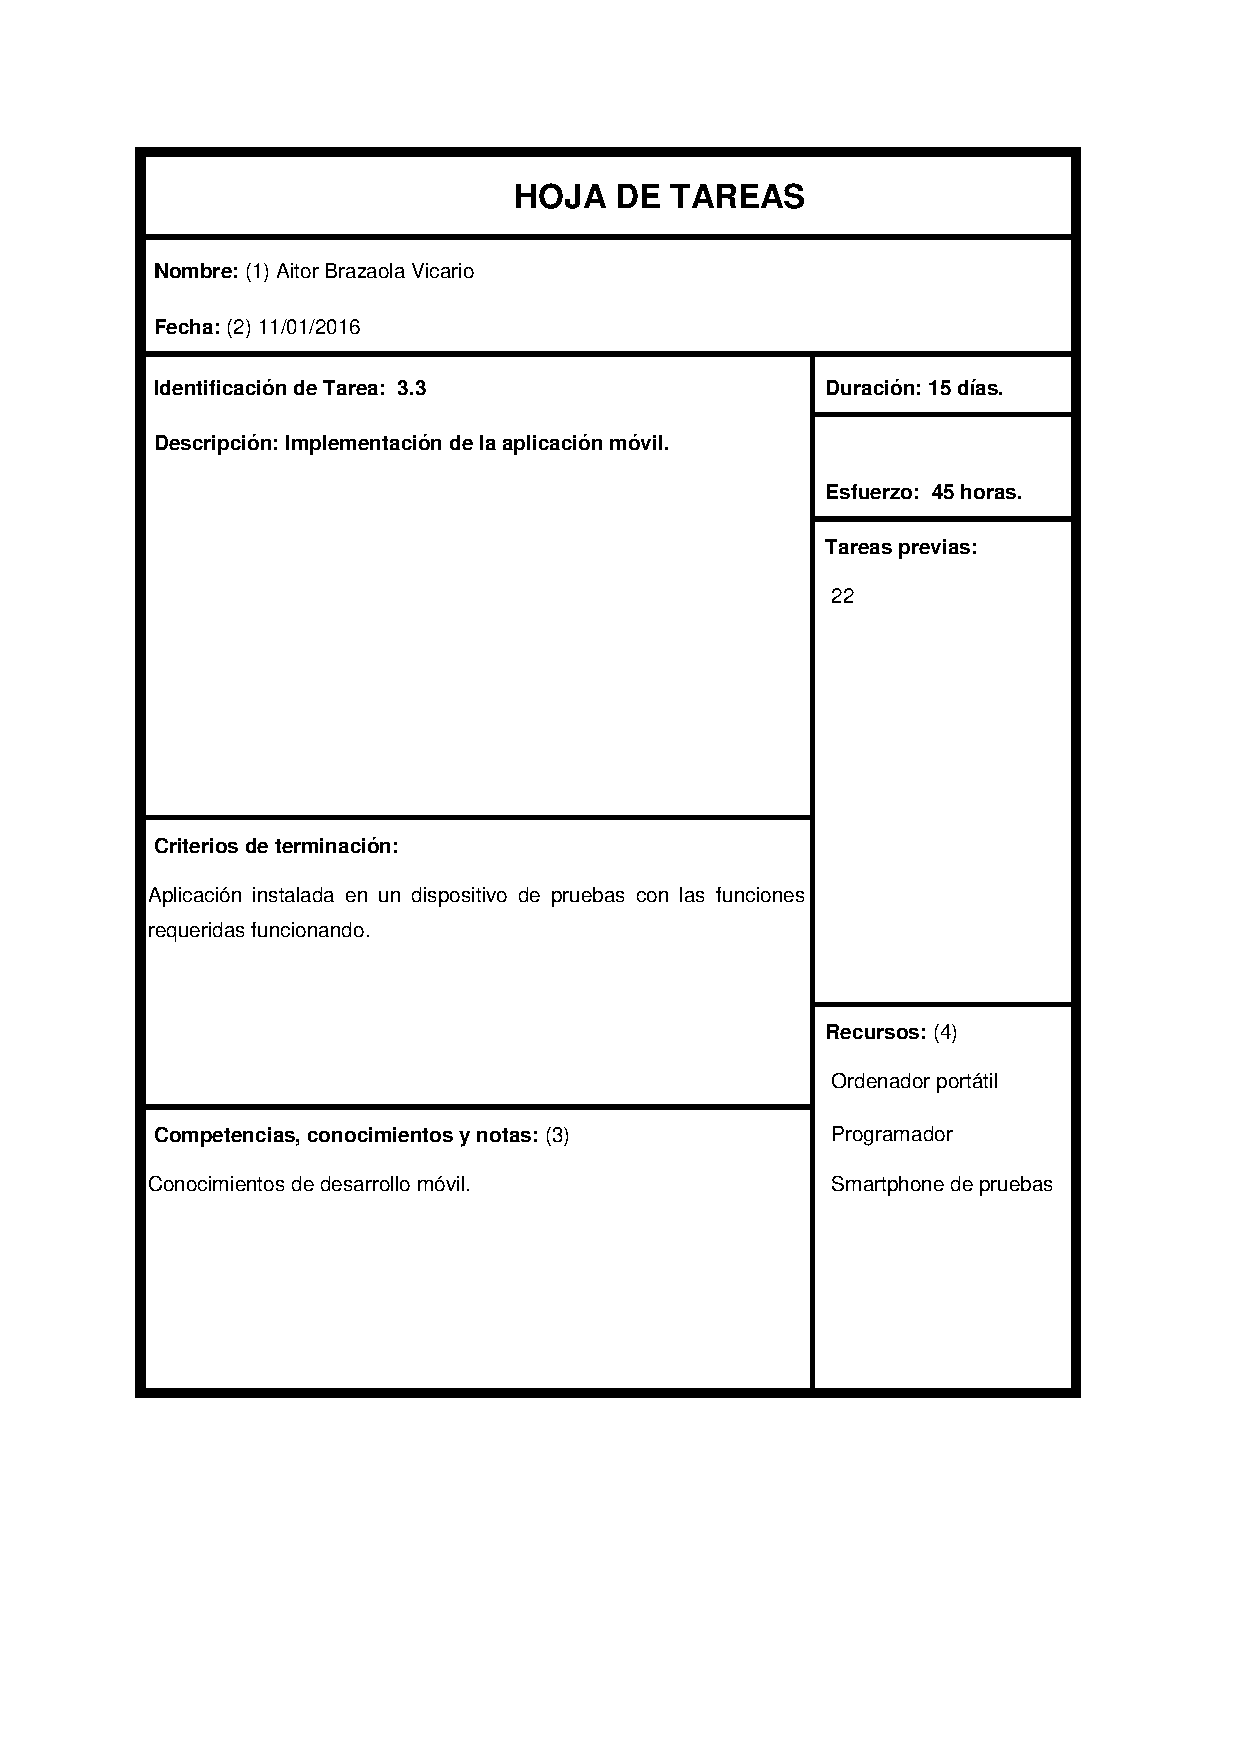
\includegraphics[width=0.9\textwidth]{fig/Tareas/33}
	\caption{Task 3.3.}
	\label{fig:t33}
\end{figure}

\begin{figure}[H]
	\centering
	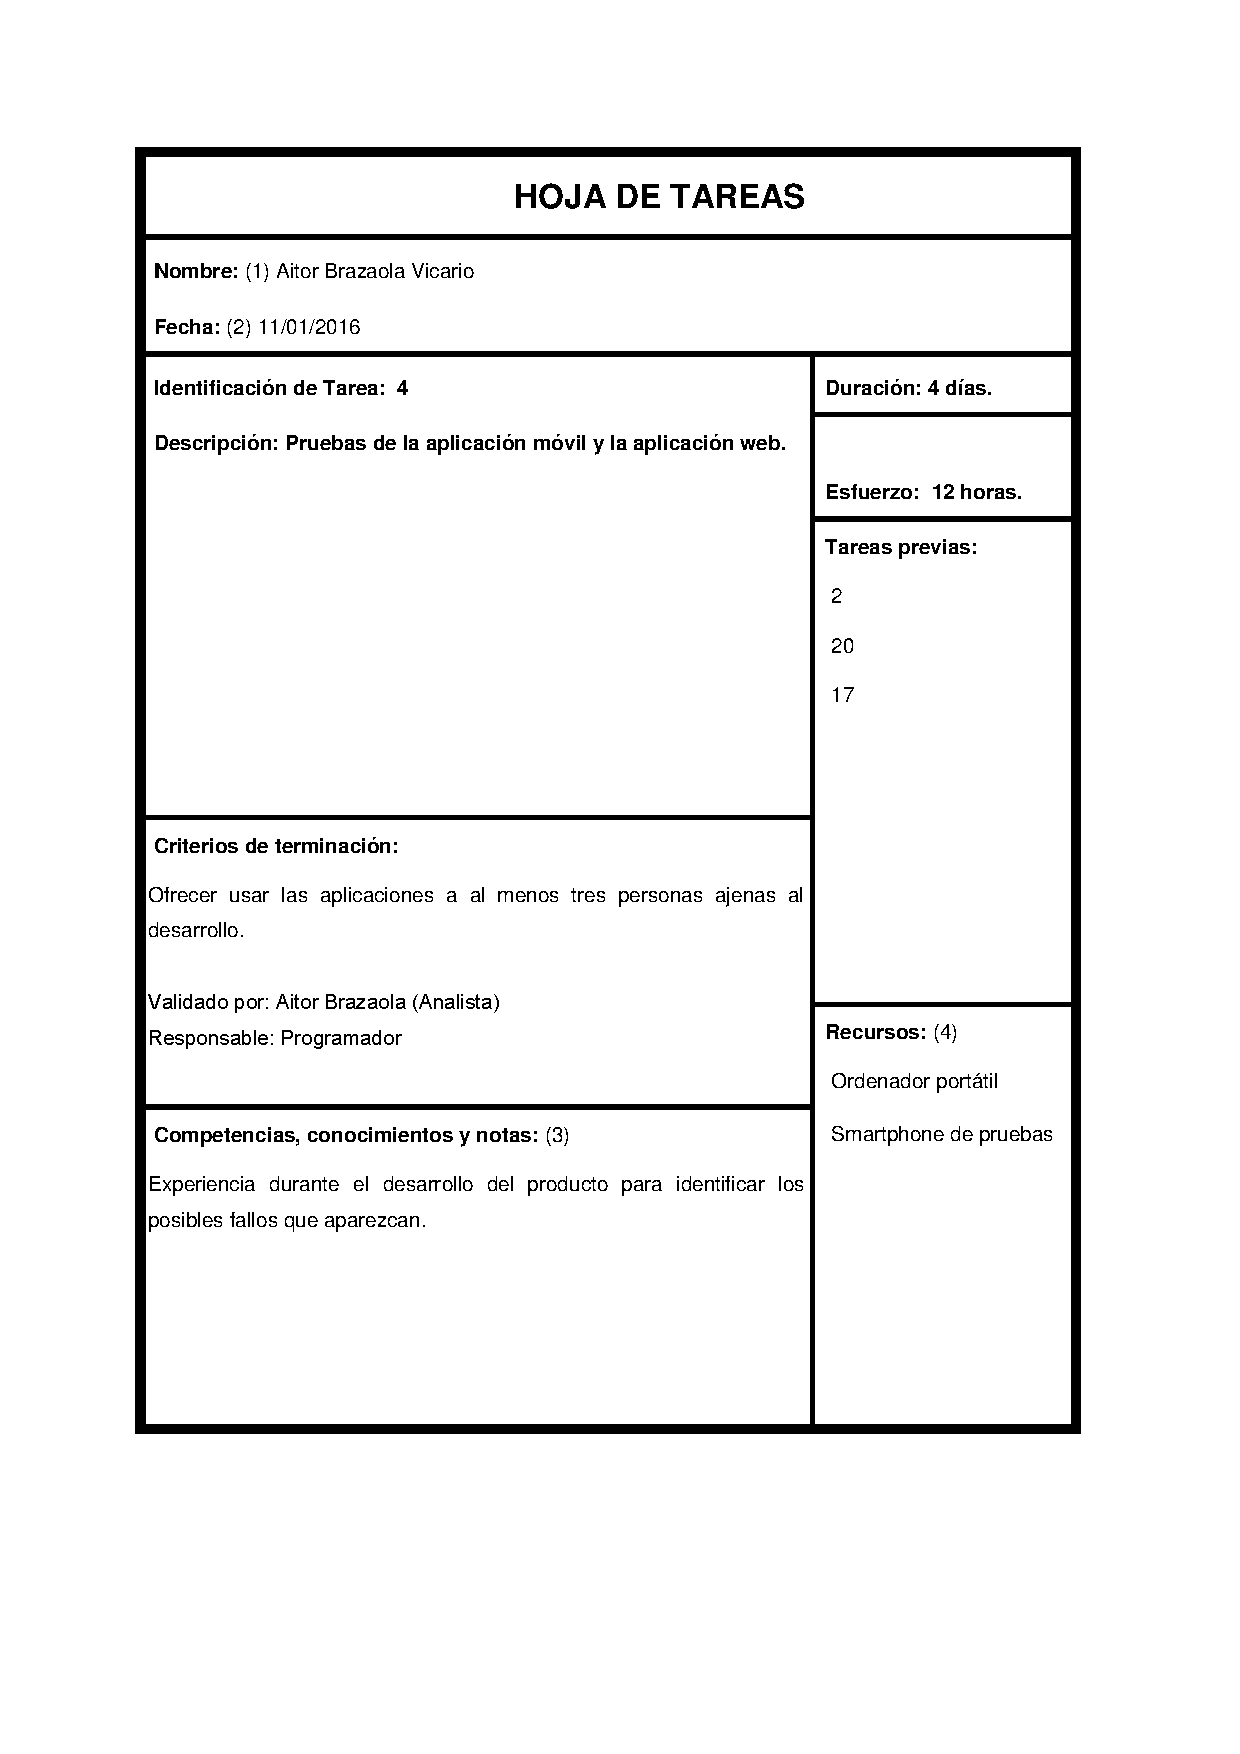
\includegraphics[width=0.9\textwidth]{fig/Tareas/4}
	\caption{Task 4.}
	\label{fig:t4}
\end{figure}
\section{Organization}
\subsection{Organizational structure}
The organization as can be seen in the figure \ref{fig:esquemaorganizacion}, is composed by the Project manager, and the student who perform the roles of programmer and designer.

\begin{figure}[h]
	\centering
	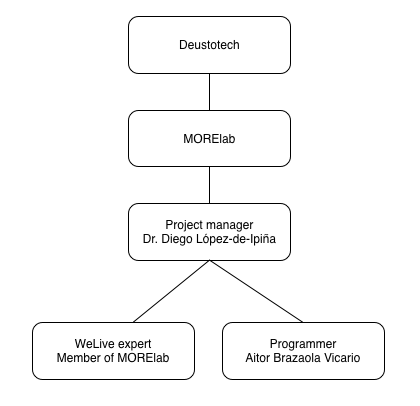
\includegraphics[width=0.7\linewidth]{fig/esquemaorganizacion}
	\caption[Organizational schema]{Organizational schema}
	\label{fig:esquemaorganizacion}
\end{figure}

Every two weeks there will be a session for reviewing the work done and the necessary changes will be assessed and if the product is already to consider as a functional unit.

\newpage
The main assistants will be the programmer and the project manager, the details exposed will be gathered in the meeting act, the template used for this proposal can be seen in the figure \ref{fig:Actareunion}, and will be prioritized over the rest of the features in the pipeline, avoiding develop in an incorrect way.

\begin{figure}[h]
	\centering
	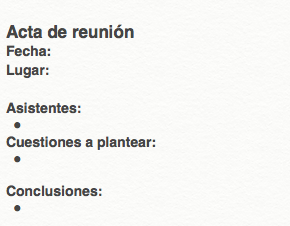
\includegraphics[width=0.7\linewidth]{fig/Actareunion}
	\caption[Template meeting act]{Template meeting act}
	\label{fig:Actareunion}
\end{figure}
\subsection{Human resources plan}
The student will be the unique physical person in the development team but will be necessary the acquisition of various roles along the project, it is true that un punctual cases can be helped by other mates of the laboratory where is working on, but the most of the project is developed by him.

Following, there are listed the main roles played by the student:

\begin{description}
	\item[Programmer:] It is responsible for creating all the logic of the program and perform the different configurations in the devices responsible for the platform work. Its functions also cover the early stages of software design, data schema creation and conduct appropriate tests to detect errors.
	
	\item[Designer:] It is commissioned to design a user interface that fits all available screens and make the application accessible to people with disabilities and ensure a satisfactory user experience and consistent navigation between different sections of the web.
\end{description}

In addition to the student, the project has its project manager who is responsible for approving all changes and proposals that the student considers interesting to improve the product, will be present at the meetings and will be responsible for marking the milestone dates.

\chapter{Planning}
\section{Precedence diagram}
\begin{figure}[H]
	\centering
	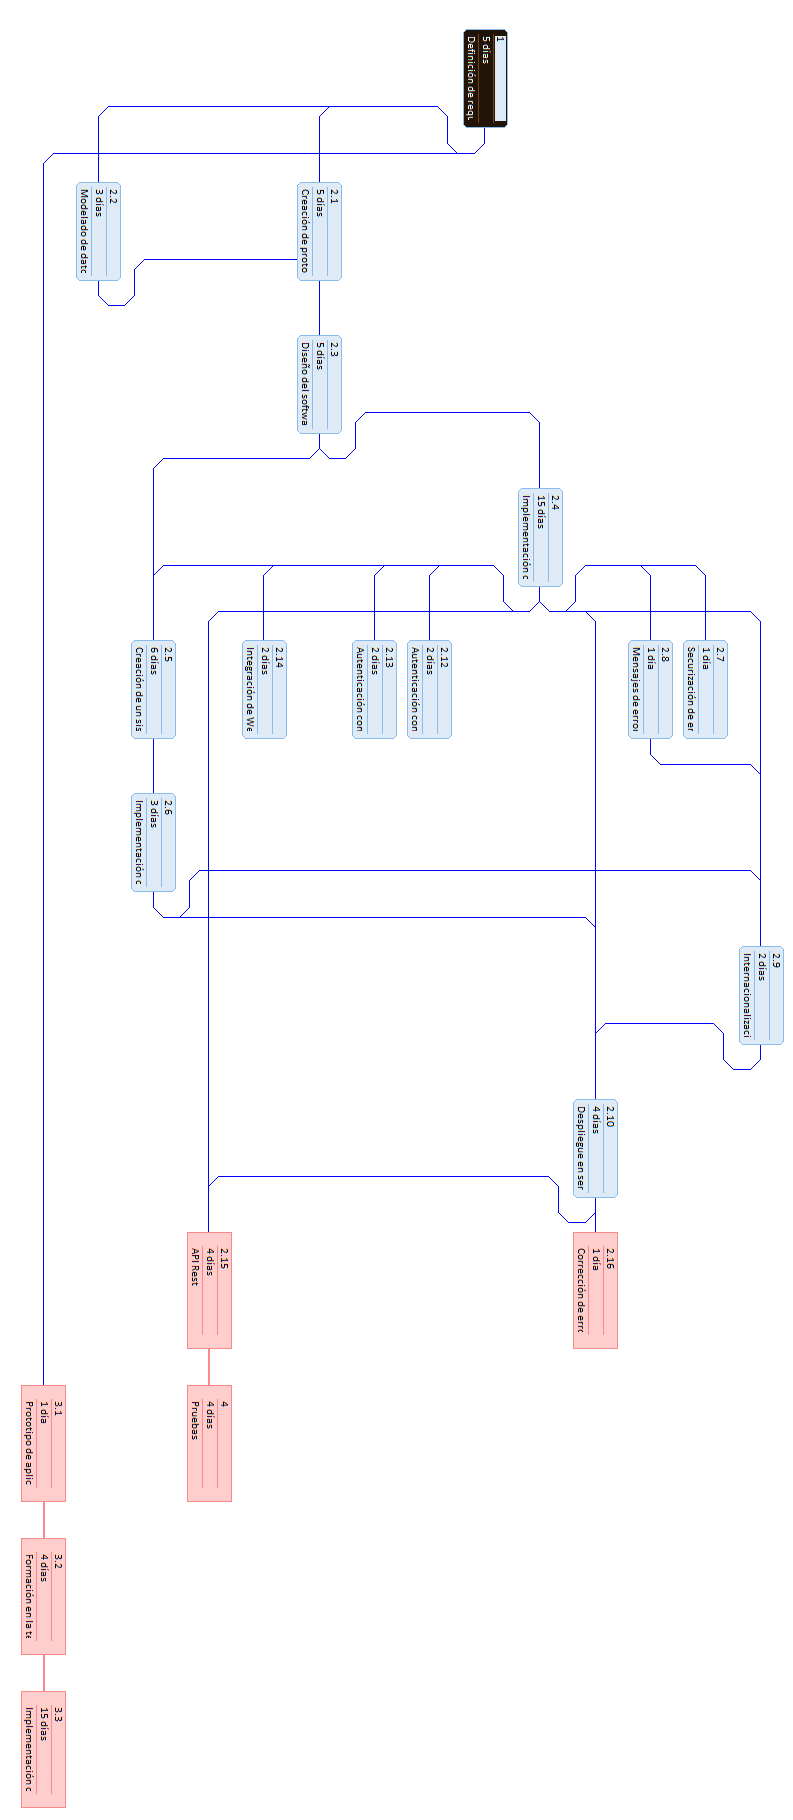
\includegraphics[width=210pt]{fig/precedencia}
	\caption{Precedence diagram}\label{fig:precedencediagram}
\end{figure}

The project development is going to happen during the working time in DeustoTech MORElab of 4 daily hours, and the team will be formed by the following actors:

\begin{description}
	\item[Programmer:] Person in charge of programming the control structures of the platform.
	\item[Designer:] Person in charge of the final appearance with the end user will interact.
	\item[Project manager:] Person in charge of monitoring the progress of the project and its organization.
	\item[Experto en plataforma WeLive:] MoreLab team member participating in the development of technical advice WeLive platform for the team.
\end{description}

\newpage
\section{GANTT diagram}
\begin{figure}[H]
	\centering
	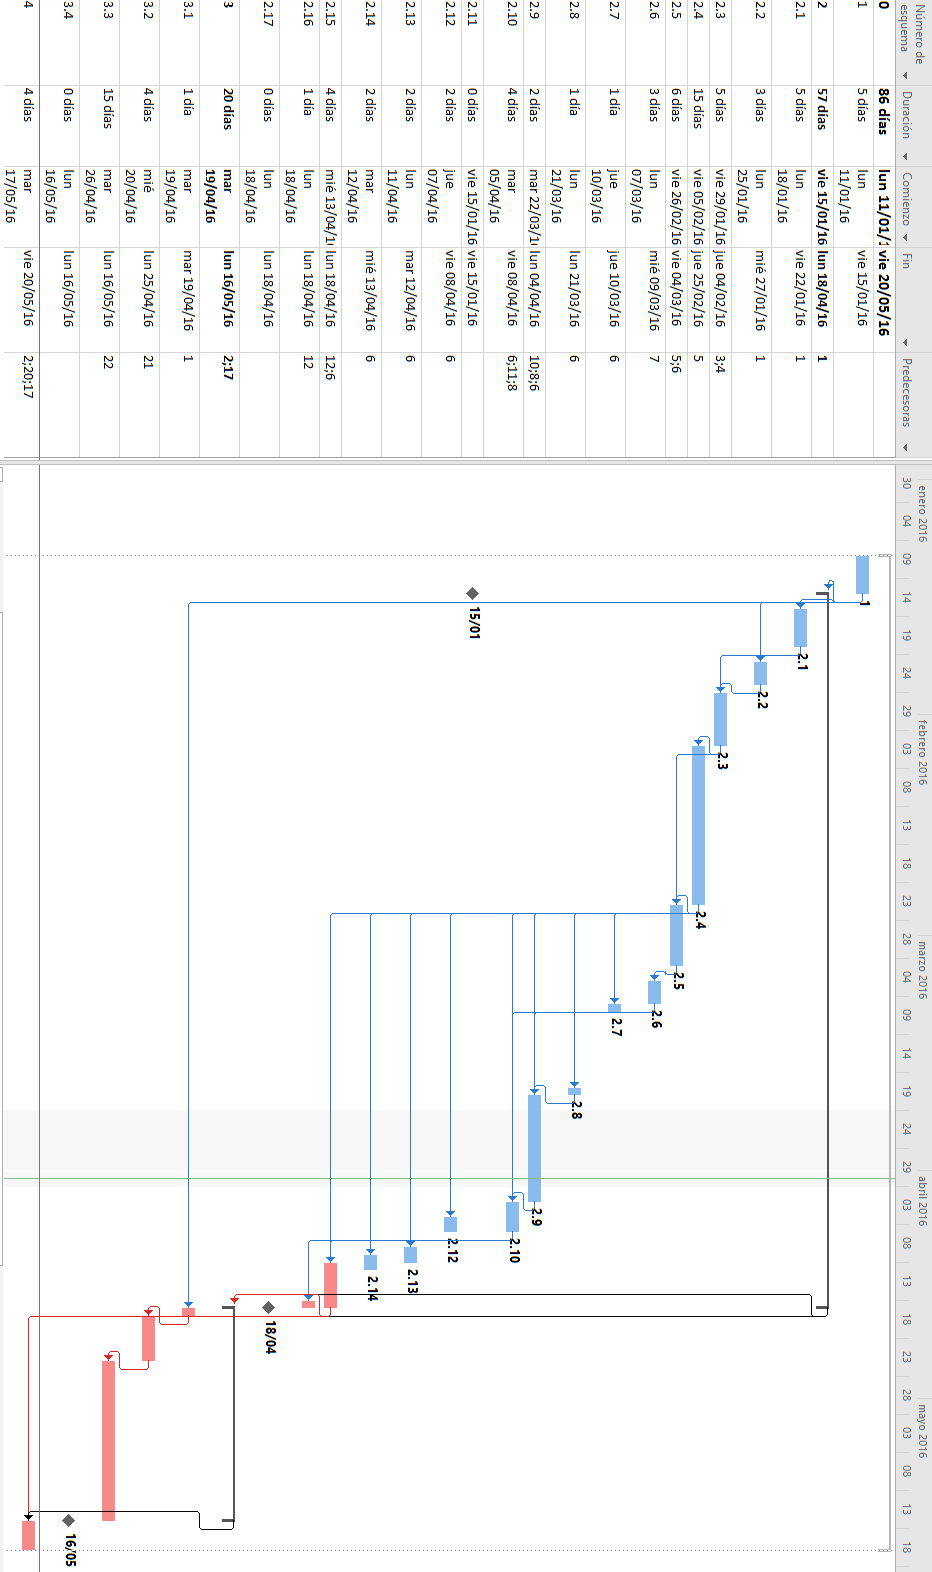
\includegraphics[width=340pt]{fig/gantt}
	\caption{GANTT diagram}\label{fig:gantt}
\end{figure}

\section{Workload estimation by profile}
The following estimation is based on the different profiles of the total 255 hours:
\begin{description}
	\item[Programmer:] 215 hours.
	\item[Designer:] 22 hours.
	\item[Project manager:] 15 hours.
	\item[WeLive platform expert:] 3 hours.
\end{description}

\begin{itemize}
	\item 1. Requirements definition: 15 hours.
	\item 2. Web application: 168 hours.
	\begin{itemize}
		\item 2.1. Web application prototype: 15 hours.
		\item 2.2. Data modeling: 9 hours.
		\item 2.3. Software design: 15 hours.
		\item 2.4. Implementation of the core features: 51 hours.
		\item 2.5. Users system creation: 18 hours.
		\item 2.6. Implementation of mail notifications: 15 hours.
		\item 2.7. Link security checks: 3 hours.
		\item 2.8. Friendly error messages: 3 hours.
		\item 2.9. Internationalization: 6 hours.
		\item 2.10. Server deployment: 12 hours.
		\item 2.13. Visual customization and logo: 6 hours.
		\item 2.14. WeLive API integration: 12 hours.
		\item 2.16. High density displays visual fixes: 3 hours.
	\end{itemize}
	\item 3. Mobile application: 60 hours.
	\begin{itemize}
		\item 3.1. Mobile application prototype: 3 hours.
		\item 3.2. Learning the selected technology for development: 12 hours.
		\item 3.3. Mobile app implementation: 45 hours.
	\end{itemize}
	\item 4. Tests: 12 hours.
\end{itemize}
\chapter{Budget}
The budget will take into account only the hours of work because the necessary equipments are already owned by the programmer and DeustoTech facilities where the project is located.

\begin{table}[H]
	\centering
	\caption{Budget by profile.}\label{tab:budgetprofile}
	\begin{tabular}{cccc}
		\toprule
		\textbf{Profile} & \emph{Workload} & \emph{Cost} & \emph{Price}\\
		\midrule
		Programmer  & 255 h.     & 9€/h. & 2295€ \\
		Designer   & 22 h.     & 9€/h. & 198€ \\
		Project manager & 12 h.     & 50€/h.  & 600€ \\
		WeLive platform expert & 3 h.     & 6€/h. & 18€ \\
		TOTAL & & & 3.111€\\
		\bottomrule
	\end{tabular}
\end{table}

\chapter{Development}
The main section of the development is going to be for the web application, the part of the project with more effort, and technologies involved in development, then, the mobile application as a derivative product from the web app will be explained in detail reasoning the technologies used with their advantages and drawbacks.

Both products has been submitted to testing with collaborators and the process of the tests will be detailed, finally a user manual will be included for helping to use all functionality implemented by the platform.
\section{Web application}
\subsection{Issue management}
All changes and requests received during the development process of the project will be managed through the following procedure:
\begin{enumerate}
	\item Communication via electronic support of the requested modification.
	\item Request meeting with the project manager for decide if the change has to be implemented.
	\item If so, assess the technical changes required on the platform before deploying.
	\item If the changes are technically feasible and fit the budget and schedule, proceed to implementation.
	\item Modify the work plan and budget.
\end{enumerate}
\section{Responsive design and mobility}
\section{Technology}
\subsection{Hardware}
\subsection{Software}
\section{Tools}
\subsection{Code editor}
\subsection{Testing}
\subsection{Operating system}
\subsection{Version control}

\chapter{Conclusions and future work}
\section{Data mining}
\section{Conclusions}
\section{Future lines of work}

\chapter{Acknowledgments}

\chapter{Agradecimientos}

\printbibliography[heading=bibintoc]

\appendix

\backmatter

\end{document}
